\documentclass[11pt]{article}
%%%%%%%%%%%%%%%%%%%%%%%%%%%%%%%%%%%%%%%%%%%%%%%%%%%%%%%%%%%%%%%%%%%%%%%%%%%%%%%%
%%%%%%%% USER DEFINED PACKAGES:
\usepackage{tgtermes}
\usepackage{geometry}
\geometry{left=3.2cm, right=2cm, top=2.4cm, bottom=2.4cm, footskip=30pt}
\usepackage[utf8]{inputenc} 
\usepackage[T1]{fontenc}     
\usepackage[frenchb]{babel}
\usepackage{amsmath}
\usepackage{amssymb}
\usepackage{gensymb}
\usepackage{epsfig}
\usepackage{epstopdf}
\usepackage{tabularx}
\usepackage{float}
\usepackage{fancyvrb}
\usepackage{subcaption}
%\usepackage{subfloat}
\usepackage{soul}% http://ctan.org/pkg/soul
\usepackage{array}
\usepackage{makecell}
\setcellgapes{4pt}
\usepackage{tabularx}
\usepackage{ragged2e}
\newcolumntype{L}[1]{>{\RaggedRight\arraybackslash}p{#1}} % just a guess...
\renewcommand{\arraystretch}{2.0} % this needs to occur before "\begin{tabular}"

\usepackage{tocloft}
\usepackage{titling}
\usepackage{pmboxdraw}

\usepackage{titlesec}
\setcounter{secnumdepth}{4}
\titleformat{\paragraph}
{\normalfont\normalsize\bfseries}{\theparagraph}{1em}{}
\titlespacing*{\paragraph}
{0pt}{3.25ex plus 1ex minus .2ex}{1.5ex plus .2ex}

\usepackage{listings} 
\usepackage{minted}

\lstset{% 
  showstringspaces=false,
  columns=fullflexible,
  showspaces=false,
  basicstyle=\footnotesize\ttfamily, 
  breaklines=true,
  columns=fullflexible,
  keepspaces=true,
  escapeinside = ||,
  breakindent=0pt} 
\lstnewenvironment{example}{}{} 

\usepackage{xcolor}
\definecolor{mygreen}{RGB}{8,217,42}
\definecolor{myred}{RGB}{243,132,184}
\definecolor{lbcolor}{rgb}{0.96,0.96,0.96}

\usepackage{hyperref}
\usepackage[hang,flushmargin]{footmisc} 
\setlength{\parindent}{0cm}




\usepackage{fancyhdr}
\usepackage{lastpage}
 \pagestyle{fancy}
\fancyhf{}
\fancyhead[LE,RO]{\slshape\nouppercase{\rightmark}}
\fancyfoot[LE,RO]{Plugin QGIS 3}
\fancyfoot[CO]{\thepage/\pageref{LastPage}}
\fancyfoot[RE,LO]{HES d'été 2024}

 
 

\graphicspath{{images/}}

\AtBeginDocument{
	\renewcommand{\listfigurename}{Liste des figures}
	\renewcommand{\tablename}{\textsc{Tableau}}
}

%%%%%%%%%%%%%%%%%%%%%%%%%%%%%%%%%%%%%%%%%%%%%%%%%%%%%%%%%%%%%%%%%%%%%%%%%%%%%%%%
\pretitle{%
  \LARGE
  
\includegraphics[width=5cm]{HEIG-VD_logotype-baseline_rouge-rvb.png}\\%HEIG-VD_Logo_83x25_CMJN_ROUGE.png}\\
  \begin{center}
}
\posttitle{\end{center}}

\title{
\vspace{-0mm}\Huge{Introduction à la création de plugins sous QGIS 3}\\ 
\vspace*{0.64em}
*\quad*\quad*  \\
\vspace*{0.64em}
\LARGE{HES d'été }
}

\input{auth}


\setlength{\cftbeforetoctitleskip}{2em} % TOC: Table of Contents
\setlength{\cftbeforeloftitleskip}{2em} % LOF: Listing of Figures
\setlength{\cftbeforelottitleskip}{2em} % LOT: Listing of Tables

%%%%%%%%%%%%%%%%%%%%%%%%%%%%%%%%%%%%%%%%%%%%%%%%%%%%%%%%%%%%%%%%%%%%%%%%%%%%%%%%

\begin{document}
\clearpage
\maketitle

\begin{center}
\begin{figure}[H]
    \centering
    \begin{subfigure}[t]{0.44\textwidth}
    	\centering		
        \raisebox{-8pt}[0pt][0pt]{
\includegraphics[width=6cm]{qgis-logo_anita02.png}}
    \end{subfigure}%
    \raisebox{24pt}[0pt][0pt]{\Huge\&\normalsize}
    \begin{subfigure}[t]{0.44\textwidth}
        \centering
        
\includegraphics[width=6cm]{python-logo-master-v3-TM-flattened.png}
    \end{subfigure}
\end{figure}
\end{center}
\thispagestyle{empty}

\clearpage % end title page
\begingroup
  \thispagestyle{empty}
  \null
  \newpage
\endgroup

\vspace*{-4.4em}
\tableofcontents
%\newpage
\vspace*{-1.2em}
\listoffigures
\vspace*{-1.2em}
\listoftables



\newpage{}

\pagestyle{fancy}
%%%%%%%%%%%%%%%%%%%%%%%%%%%%%%%%%%%%%%%%%%%%%%%%%%%%%%%%%%%%%%%%%%%%%%%%%%%%%%%%
% Chapter 1
%%%%%%%%%%%%%%%%%%%%%%%%%%%%%%%%%%%%%%%%%%%%%%%%%%%%%%%%%%%%%%%%%%%%%%%%%%%%%%%%

%%%%%%%%%%%%%%%%%%%%%%%%%%%%%%%%%%%%%%%%%%%%%%%%%%%%%%%%%%%%%%%%%%%%%%%%%%%%%%%%
\section{Introduction à Python dans QGIS}
\label{Introduction}
%%%%%%%%%%%%%%%%%%%%%%%%%%%%%%%%%%%%%%%%%%%%%%%%%%%%%%%%%%%%%%%%%%%%%%%%%%%%%%%%
\textbf{Avertissement préalable}\\\vspace*{-0.4em}

Dans sa version 2.x QGIS permettait l'utilisation du langage de programmation Python 2.7.
Dans sa version 3.x QGIS utilise dorénavant Python >=3.5.
Les deux versions majeures de Python ne sont pas entièrement compatibles, c'est pourquoi, un plugin qui aurait été écrit en Python 2.7 pour QGIS 2.18 par exemple, devra être traduit en Python 3.x pour être porté sur la version 3.x de QGIS.\\

Le présent document survole brièvement l'utilisation de Python (3.x) et le développement de plugins pour la version 3 de QGIS. \\
La version de Python embarquée dans l'installation de QGIS se découvre en parcourant le menu \og{}\texttt{Aide > À propos}\fg{} de QGIS.\\


\textbf{L'API Python de QGIS}\\\vspace*{-0.4em}

Dans le cadre de la création de nouveaux plugins, l'API de QGIS est très souvent appelée. Une API est une interface de programmation. C'est grâce à elle qu'il est possible d'interagir avec les objets d'un programme depuis un autre; dans notre cas, il nous sera possible d'interagir avec les couches, les objets et l'interface de QGIS directement depuis Python. \\

Ce chapitre permet donc de se familiariser avec cette API à travers la console Python de QGIS. D'ailleurs, par l'intermédiaire de cette console, il est possible d'enregistrer les scripts Python afin de pouvoir les réutiliser ultérieurement (par exemple dans un plugin). 


%%%%%%%%%%%%%%%%%%%%%%%%%%%%%%%%%%%%%%%%
\subsection{Présentation de la console Python dans QGIS}
\label{Presentation}
%%%%%%%%%%%%%%%%%%%%%%%%%%%%%%%%%%%%%%%%

La console Python dans QGIS se présente comme suit :


\begin{figure}[H]
    \centering
    \begin{subfigure}[t]{0.70\textwidth}
		
        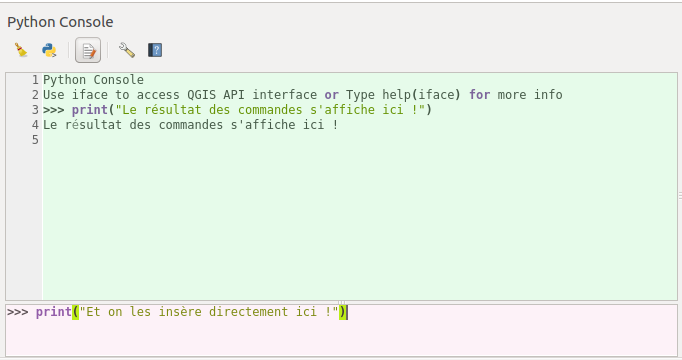
\includegraphics[width=1\textwidth]{python_console_qgis3_colored.png}
\caption{La zone figurée en \colorbox{mygreen!32}{vert} correspond à la \textbf{sortie}; le résultat des commandes s'affiche ici. La zone figurée en \colorbox{myred!32}{rouge} correspond à l'\textbf{invite de commande}, il s'agit de l'espace de \textbf{saisie} des commandes par l'utilisateur.\\
\underline{\smash{Remarque}}: l'effacement de la console n'efface que l'affichage de la sortie; les variables restent en mémoire!}\label{fig1:consolepython}
    \end{subfigure}%
    ~
    \begin{subfigure}[t]{0.32\textwidth}
        \hspace*{2em}
        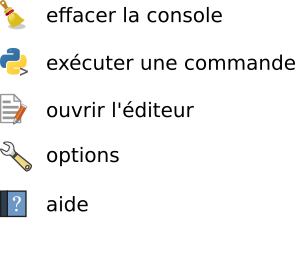
\includegraphics[width=0.8\textwidth]{drawing_console.png}
        \caption{Légende de quelques boutons.}\label{fig1:icons}
    \end{subfigure}
    \label{fig1}
    \caption{La console Python de QGIS.}
\end{figure}




\newpage{}
L'éditeur, qui s'ouvre avec le bouton 
\includegraphics[width=1em]{iconShowEditorConsole.png}, se présente quant à lui de la manière suivante :

\begin{figure}[H]
    \centering
    \begin{subfigure}[t]{0.70\textwidth}
		
        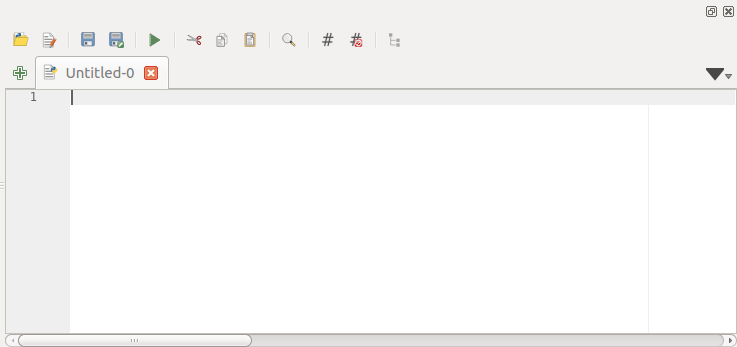
\includegraphics[width=1\textwidth]{python_editor_qgis3.png}
\caption{Créer et sauvegarder ses scripts Python est possible directement dans QGIS grâce à l'\textbf{éditeur}.}\label{fig2:consolepython}
    \end{subfigure}%
    ~
    \begin{subfigure}[t]{0.32\textwidth}
        \hspace*{-1em}
        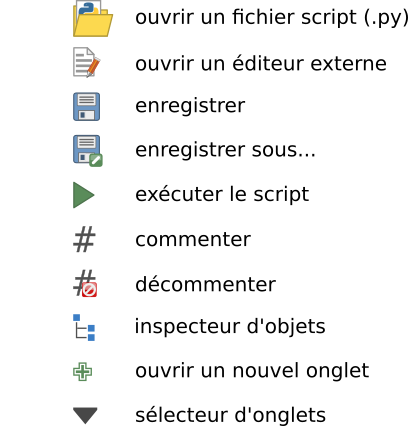
\includegraphics[width=1\textwidth]{drawing_editor.png}
        \caption{Légende de quelques boutons.}\label{fig2:icons}
    \end{subfigure}
    \label{fig2}
    \caption{L'éditeur de scripts Python de QGIS.}
\end{figure}


%%%%%%%%%%%%%%%%%%%%%%%%%%%%%%%%%%%%%%%%
\subsection{Exercice avec la console Python}
\label{Exercice}
%%%%%%%%%%%%%%%%%%%%%%%%%%%%%%%%%%%%%%%%

\subsubsection{Contexte}
Cet exercice permet de lire un fichier au format "ESRI Shapefile" (\texttt{SHP}), de récupérer non seulement les attributs, mais également la géométrie (latitude et longitude), d'afficher ces différentes caractéristiques et de les écrire dans un fichier texte (\texttt{TXT}). De plus, il permet d'écrire un nouveau fichier \texttt{SHP} en projetant les données dans un autre système de coordonnées. 

\subsubsection{Données}
Les données utilisées dans le cadre de cet exercice sont les points d'intérêt d'OpenStreetMap (\url{http://download.geofabrik.de}) au format \texttt{SHP}. 

\subsubsection{Marche à suivre}

\begin{enumerate}\itemsep0.4em
\item Préparations préalables:
\begin{itemize}\itemsep0.2em
\renewcommand\labelitemi{\---}
\item Créer un nouveau dossier à votre nom pour ce cours sur le disque \texttt{D:} de l'ordinateur : \og{}temp\_votreNom\fg{}
\item Télécharger dans votre dossier les données suisses d'OpenStreetMap au format \texttt{SHP} à partir du lien suivant : 
\vspace*{-0.4em}
\begin{center}

\includegraphics[width=1.64cm]{osm.png}\\
\url{http://download.geofabrik.de}
\end{center}
\vspace*{0.4em}

\item Ouvrir QGIS et créer un nouveau projet
\item Ajouter la couche des points d'intérêt (\og{}\texttt{gis\_osm\_pois\_free\_1.shp}\fg{}) dans ce nouveau projet à partir du menu \og{}\texttt{Couche > Ajouter une couche > Ajouter une couche vectorielle}\fg{} : 

\vspace*{-0.4em}
\begin{figure}[H]
\centering
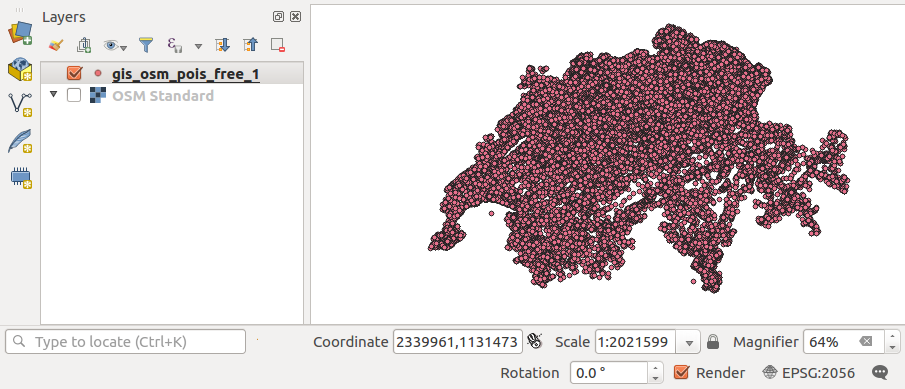
\includegraphics[width=0.8\textwidth]{osm_data.png}
\vspace*{-0.64em}
\caption{Les données des points d'intérêt (\emph{poi}) OSM de la Suisse dans QGIS.}
\label{osmdata}
\end{figure}
\vspace*{0.4em}

\item Sélectionner un échantillon d'environ 300 à 500 points dans la ville d'Yverdon-les-Bains
\item Enregistrer la sélection au format \texttt{SHP} sous un nouveau nom (par ex. : \og{}\texttt{poi\_selection}\fg{})
\item Supprimer maitnenant la couche de tous les points d'intérêt
\item Ajouter la couche précédemment créée (échantillon des points d'intérêt) 
\end{itemize}
\item Ouvrir la console Python de QGIS : menu \og{}\texttt{Extension > Console Python}\fg{}.\\
\underline{\smash{Remarque}}: dès à présent, les différentes étapes seront effectuées uniquement par l'intermédiaire de la console Python ! 
\item Récupérer la couche active de ce projet QGIS (ndlr : la couche échantillon des points d'intérêt. Cette couche doit impérativement être sélectionnée dans la table des matières de QGIS) grâce à la fonction \texttt{activeLayer()} :
\vspace*{-1em}
\begin{center}
\begin{minipage}[t]{0.32\textwidth}
\begin{minted}[frame=single,
  escapeinside=||,
  mathescape,
  %bgcolor=lbcolor,
  linenos,
  numbersep=5pt,
  fontsize=\small,
  framesep=1mm]{python3}
layer = iface.activeLayer() 
\end{minted}
\end{minipage}
\end{center}
\vspace*{1em}

\underline{\smash{Remarque}}:
\begin{itemize}\itemsep0.2em
\renewcommand\labelitemi{\--}
\item Pour exécuter cette commande depuis la console Python : utiliser la touche \og{}Enter\fg{} du clavier. 
\item \og{}\texttt{iface}\fg{} est un objet de la classe \texttt{QgsInterface} qui permet d'accéder au canevas de carte, aux menus, aux barres d'outils, etc. 
\item Ici, \og{}\texttt{layer}\fg{} est le nom de la variable dans lequel le résultat de la fonction \texttt{activeLayer()} est stocké. Il est donc possible de nommer cette variable autrement. 
\item \og{}\texttt{layer}\fg{} renvoie à un objet de la classe \og{}\texttt{QgsVectorLayer}\fg{} :
\vspace*{-0em}
\begin{center}
\begin{minipage}[t]{0.66\textwidth}
\begin{minted}[frame=single,
  escapeinside=||,
  mathescape,
  %bgcolor=lbcolor,
  linenos,
  numbersep=5pt,
  fontsize=\small,
  framesep=1mm]{python3}
<qgis._core.QgsVectorLayer object at 0x0000000001BF57D9>
\end{minted}
\end{minipage}
\end{center}
\vspace*{1em}

\end{itemize}

\item Récupérer tous les différents éléments (\emph{features}), c'est-à-dire les différents points d'intérêt de la couche en utilisant la méthode \texttt{getFeatures()} : 
\vspace*{-1em}
\begin{center}
\begin{minipage}[t]{0.24\textwidth}
\begin{minted}[frame=single,
  escapeinside=||,
  mathescape,
  %bgcolor=lbcolor,
  linenos,
  numbersep=5pt,
  fontsize=\small,
  framesep=1mm]{python3}
layer.getFeatures()
\end{minted}
\end{minipage}
\end{center}
\vspace*{1em}


\includegraphics[scale=1]{tip_l.png} \underline{\smash{Astuce}}: pour afficher les différentes variables et méthodes possibles d'un objet, il est possible d'utiliser la fonction \texttt{dir()}. Exemple : 
\vspace*{-1em}
\begin{center}
\begin{minipage}[t]{0.14\textwidth}
\begin{minted}[frame=single,
  escapeinside=||,
  mathescape,
  %bgcolor=lbcolor,
  linenos,
  numbersep=5pt,
  fontsize=\small,
  framesep=1mm]{python3}
dir(layer)
\end{minted}
\end{minipage}
\end{center}
%\vspace*{1em}









\newpage{}
$\Rightarrow$ La fonction \texttt{getFeatures()} renvoie un objet de type \textbf{itérateur} : 
\vspace*{-1em}
\begin{center}
\begin{minipage}[t]{0.72\textwidth}
\begin{minted}[frame=single,
  escapeinside=||,
  mathescape,
  %bgcolor=lbcolor,
  linenos,
  numbersep=5pt,
  fontsize=\small,
  framesep=1mm]{python3}
<qgis._core.QgsFeatureIterator object at 0x0000000001BF57E18>
\end{minted}
\end{minipage}
\end{center}
\vspace*{1em}

Pour pouvoir récupérer les différents éléments de la couche, il est donc nécessaire d'effectuer une \textbf{itération }sur cet objet, c'est-à-dire une \textbf{boucle}. 



\item Afficher les différents éléments de cette couche en ajoutant une boucle sur la fonction \texttt{getFeatures()} : 
\vspace*{-2em}
\begin{center}
\begin{minipage}[t]{0.42\textwidth}
\begin{minted}[frame=single,
  escapeinside=||,
  mathescape,
  %bgcolor=lbcolor,
  linenos,
  numbersep=5pt,
  fontsize=\small,
  framesep=1mm]{python3}
for feature in layer.getFeatures():
    print(feature)
\end{minted}
\end{minipage}
\end{center}
\vspace*{1em}


\includegraphics[scale=1]{warningt.png} \underline{\smash{Attention}}: il est nécessaire d'\textbf{indenter} la deuxième ligne afin que Python sache que cette ligne se trouve dans la boucle. Dans la console Python, l'indentation s'effectue avec quatre espaces. 

\underline{\smash{Remarque}}:
\begin{itemize}\itemsep0.2em
\renewcommand\labelitemi{\--}
\item Lorsque l'\textbf{invite de commande} de la console présente \og{}... \fg{} au lieu de \og{} >{}>{}>{} \fg{}, cela signifie qu'elle est en attente de code (par exemple : en attente de la fermeture d'une boucle) : 

\vspace*{-0.4em}
\begin{figure}[H]
\centering
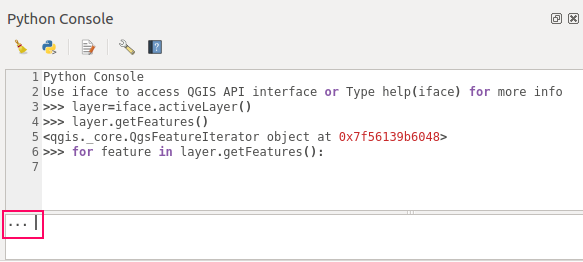
\includegraphics[width=0.64\textwidth]{prompt_wait.png}
\vspace*{-0.64em}
\caption{Invite de commande en attente de la suite d'une boucle ouverte...}
\label{prompt}
\end{figure}
\vspace*{0.4em}

\item Pour clore la boucle : appuyer sur la touche \og{}Enter\fg{}
\end{itemize}




\item À partir du résultat précédent : afficher uniquement le nom de chaque élément (colonne \og{}name\fg{}) : 
\vspace*{-1em}
\begin{center}
\begin{minipage}[t]{0.42\textwidth}
\begin{minted}[frame=single,
  escapeinside=||,
  mathescape,
  %bgcolor=lbcolor,
  linenos,
  numbersep=5pt,
  fontsize=\small,
  framesep=1mm]{python3}
for feature in layer.getFeatures():
    print(feature['name'])
\end{minted}
\end{minipage}
\end{center}
\vspace*{1em}

$\Rightarrow$ \underline{\smash{Résultats}}: la liste des noms s'affiche dans la console.

\vspace*{1em}
\underline{\smash{Remarque}}:
\begin{itemize}\itemsep0.2em
\renewcommand\labelitemi{\--}
\item \og{}\texttt{feature['name']}\fg{} peut être affecté à une nouvelle variable (par exemple : \texttt{fname}).
\item Selon le nombre d'éléments qui a été précédemment sélectionné, l'affichage peut prendre plus ou moins de temps. 
\end{itemize}

\item Récupérer la géométrie de chaque élément grâce à la méthode \texttt{geometry()} et afficher les géométries sous forme de paires de coordonnées grâce à la méthode \texttt{asPoint()} : 
\vspace*{-1em}
\begin{center}
\begin{minipage}[t]{0.42\textwidth}
\begin{minted}[frame=single,
  escapeinside=||,
  mathescape,
  %bgcolor=lbcolor,
  linenos,
  numbersep=5pt,
  fontsize=\small,
  framesep=1mm]{python3}
for feature in layer.getFeatures():
    geom = feature.geometry()
    print(geom.asPoint())
\end{minted}
\end{minipage}
\end{center}
%\vspace*{1em}






\newpage{}
\underline{\smash{Remarque}}:
\begin{itemize}\itemsep0.2em
\renewcommand\labelitemi{\--}
\item Pour récupérer uniquement la coordonnée x ou y : utiliser la méthode \texttt{x()} ou \texttt{y()} directement après \texttt{asPoint()}. 
\item Il est possible d'ajouter du texte dans l'affichage de la fonction \texttt{print()} :
\vspace*{-0.64em}
\begin{center}
\begin{minipage}[t]{0.40\textwidth}
\begin{minted}[frame=single,
  escapeinside=||,
  mathescape,
  %bgcolor=lbcolor,
  linenos,
  numbersep=5pt,
  fontsize=\small,
  framesep=1mm]{python3}
print("The layer object: ", layer)
\end{minted}
\end{minipage}
\end{center}
\vspace*{1em}

\underline{\smash{Résultat}}:
\vspace*{-0.64em}
\begin{center}
\begin{minipage}[t]{0.88\textwidth}
\begin{minted}[frame=single,
  escapeinside=||,
  mathescape,
  %bgcolor=lbcolor,
  linenos,
  numbersep=5pt,
  fontsize=\small,
  framesep=1mm]{python3}
The layer object: <qgis._core.QgsVecteorLayer object at 0x0000000001BDEE400>
\end{minted}
\end{minipage}
\end{center}
\vspace*{1em}



\includegraphics[scale=1]{warningt.png} \underline{\smash{Attention}}: les différents éléments sont séparés par des virgules. 

\end{itemize}


\item Effectuer un peu de mise en page dans la fonction \texttt{print} afin d'obtenir un résultat semblable à celui-ci : 
\vspace*{-1em}
\begin{center}
\begin{minipage}[t]{0.76\textwidth}
\begin{minted}[frame=single,
  escapeinside=||,
  mathescape,
  %bgcolor=lbcolor,
  linenos,
  numbersep=5pt,
  fontsize=\small,
  framesep=1mm]{bash}
C&A with coord X = 6.6400168 and coord Y = 46.7792502
CFF with coord X = 6.6408634 and coord Y = 46.7814805
Vierino Lauria with coord X = 6.6402715 and coord Y = 46.779728
Shop Express with coord X = 6.641174 and coord Y = 46.7814
NULL with coord X = 6.6405565 and coord Y = 46.7796104
\end{minted}
\end{minipage}
\end{center}
\vspace*{1em}

\underline{\smash{Remarque}}: la console Python est utile pour tester quelques bouts de code, mais cela devient difficile lorsqu'on souhaite tester 100 lignes de code d'affilée (par exemple lorsqu'il y a de multiples boucles, parfois imbriquées). C'est pourquoi, l'\textbf{éditeur} de la console Python sera utilisé pour la suite de cet exercice. 


\item Ouvrir l'éditeur de la console Python à l'aide du bouton correspondant ( 
\includegraphics[width=1em]{iconShowEditorConsole.png} ) depuis la \textbf{console} Python.






\item Enregistrer un nouveau fichier Python d'\textbf{extension} \texttt{.py} dans votre dossier sur le disque \texttt{D:} à partir du bouton correspondant ( 
\includegraphics[width=1em]{mActionFileSaveAs.png} ) qui se trouve dans l'\textbf{éditeur}. 

\underline{\smash{Remarque}}:
\begin{itemize}\itemsep0.2em
\renewcommand\labelitemi{\--}
\item À cet effet, le raccourci clavier \og{}\texttt{CTRL+S}\fg{} ne fonctionne malheureusement pas, il faut impérativement cliquer sur l'icône adéquate.
\item %Avant de pouvoir enregistrer le fichier Python, QGIS demande d'enregistrer le projet QGIS en lui-même. Si le projet n'avait pas déjà été enregistré. Il est donc nécessaire d'effectuer deux enregistrements simultanés. 
L'icône d'entregistrement devient grise une fois celui-ci effectué ( 
\includegraphics[width=1em]{mActionFileSave_gray.png} ).
\item Il faut absolument éviter d'insérer des caractères spéciaux (par ex. accentués) dans le code.
\item Dans le script Python, il est possible d'ajouter des commentaires (fig.\,\ref{comment}) avec le symbole dièse \og{}\#\fg{} en début de ligne. A cet effet, le symbole peut être ajouté manuellement (avec la touche correspondante du clavier) ou avec le bouton 
\includegraphics[width=1em]{iconCommentEditorConsole.png}.
\vspace*{-0.4em}
\begin{figure}[H]
\centering
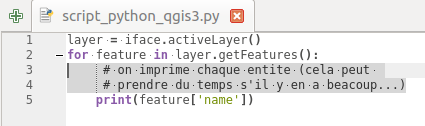
\includegraphics[width=0.44\textwidth]{comment.png}
\vspace*{-0.64em}
\caption{Deux lignes de commentaires décrivant le code dans un script Python.}
\label{comment}
\end{figure}
\vspace*{-1em}

\end{itemize}


\item Copier le code précédemment créé avec la mise en forme de la sortie. \\
Ne pas oublier de \textbf{régulièrement enregistrer} le script Python !\\ 






\newpage{}
\underline{\smash{Remarque}}: lorsqu'une boucle ou une condition est par exemple créée, l'\textbf{indentation} est \textbf{automatiquement} effectuée par l'\textbf{éditeur}. Si besoin, 4 espaces (ou une tabulation) peuvent être utilisées pour effectuer cette indentation dans l'éditeur de la console (tout comme dans l'invite de commande).\\


\includegraphics[scale=1]{warningt.png} \underline{\smash{Attention}}: avec Python, le nombre d'espaces utilisées doit impérativement être rigoureusement le même pour tous les éléments du même niveau hiérarchique d'un bloc d'instructions !

\vspace*{0.32em}
\item \textbf{Exécuter} le script à l'aide du bouton correspondant ( 
\includegraphics[width=1em]{mActionStart.png} ). \\
Vérifier ensuite le résultat qui s'affiche dans la \textbf{console} Python.


\underline{\smash{Remarque}}: il est possible qu'il y ait des problèmes d'\textbf{encodage} notamment dans le nom des points d'intérêt. Il s'agit d'un problème lors de l'import de la couche dans QGIS et pour y remédier, il faut se rendre dans les propriétés de la couche (rappel : clic droit sur la couche dans la fenêtre \og{}\texttt{Couches}\fg{}) puis, ouvrir l'onglet \texttt{Général}. Sous la section \og{}\texttt{Source}\fg{} > sous \og{}\texttt{Encodage des données sources}\fg{} on prendra soin de choisir \og{}\texttt{UTF-8}\fg{} :
\vspace*{-0.4em}
\begin{figure}[H]
\centering
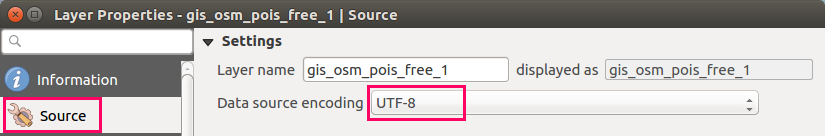
\includegraphics[width=0.8\textwidth]{utf8.png}
\vspace*{-0.4em}
\caption{Vérifier que l'encodage des caractères de la couche (onglet \og{}Source\fg{}) soit bien sur \texttt{UTF-8}.}
\label{utf8}
\end{figure}
\vspace*{-1em}


%\vspace*{0.32em}
\item Toujours depuis le script Python, c'est-à-dire depuis l'éditeur de la console Python : ajouter une \textbf{condition} dans la boucle afin de ne pas afficher les données qui n'ont pas de nom (\texttt{name = NULL}) ( 
\includegraphics[scale=1]{tip_l.png} \underline{\smash{astuce}}: utiliser simplement une condition \og{} \texttt{if}\fg{} sur le nom (\texttt{name}) pour vérifier qu'il existe bien un nom!). Le résultat devrait être semblable à celui-ci : 
\vspace*{-1em}
\begin{center}
\begin{minipage}[t]{0.76\textwidth}
\begin{minted}[frame=single,
  escapeinside=||,
  mathescape,
  %bgcolor=lbcolor,
  linenos,
  numbersep=5pt,
  fontsize=\small,
  framesep=1mm]{bash}
C&A with coord X = 6.6400168 and coord Y = 46.7792502
CFF with coord X = 6.6408634 and coord Y = 46.7814805
Vierino Lauria with coord X = 6.6402715 and coord Y = 46.779728
Shop Express with coord X = 6.641174 and coord Y = 46.7814
\end{minted}
\end{minipage}
\end{center}
\vspace*{1em}


\item Écrire le nom et les coordonnées de chaque élément dans un fichier \texttt{TXT}.\\

Pour ce faire, il est nécessaire dans un premier temps d'écrire un nouveau fichier en indiquant le chemin et le nom du fichier, ainsi que l'option \og{}\texttt{w}\fg{} pour spécifier que le fichier est ouvert en écriture (\texttt{w} pour \underline{\smash{w}}rite) : 
\vspace*{-1em}
\begin{center}
\begin{minipage}[t]{0.88\textwidth}
\begin{minted}[frame=single,
  escapeinside=||,
  mathescape,
  %bgcolor=lbcolor,
  linenos,
  numbersep=5pt,
  fontsize=\small,
  framesep=1mm]{python3}
output = open('D:/temp_votreNom/mon_projet_python_qgis3/codes/poi.txt','w')
\end{minted}
\end{minipage}
\end{center}
\vspace*{1em}

\underline{\smash{Remarque}}: si le fichier n'existe pas, il sera automatiquement créé au lancement de cette commande. \\



Indiquer préalablement l'encodage \texttt{UTF-8} grâce au code suivant : 
\vspace*{-1em}
\begin{center}
\begin{minipage}[t]{0.4\textwidth}
\begin{minted}[frame=single,
  escapeinside=||,
  mathescape,
  %bgcolor=lbcolor,
  linenos,
  numbersep=5pt,
  fontsize=\small,
  framesep=1mm]{python3}
line_encode = line.encode('utf-8')
\end{minted}
\end{minipage}
\end{center}
\vspace*{1em}

où \og{}\texttt{line}\fg{} est le nom de la variable qui contient les données :
\vspace*{-1em}
\begin{center}
\begin{minipage}[t]{0.264\textwidth}
\begin{minted}[frame=single,
  escapeinside=||,
  mathescape,
  %bgcolor=lbcolor,
  linenos,
  numbersep=5pt,
  fontsize=\small,
  framesep=1mm]{python3}
line = '%s\n' % (data)
\end{minted}
\end{minipage}
\end{center}
%\vspace*{1em}










\newpage{}
\underline{\smash{Rappel}}:\\
\vspace{0.2em}
\og{}\%s\fg{} permet d'indiquer que \og{}\texttt{data}\fg{} est une chaîne de caractères (\texttt{s} pour \underline{\smash{s}}tring). Ainsi, pour définir la variable \og{}\texttt{data}\fg{}, vous pouvez par exemple concaténer différentes chaînes de caractères (\emph{string}) à l'aide du symbole \og{}+\fg{}. Pour transformer des entiers ou des nombres à virgules en chaînes de caractères : utiliser la fonction \texttt{str()}.

\vspace{0.64em}
\hspace*{2em}
\begin{minipage}[t]{0.88\textwidth}
\underline{\smash{Exemples pratiques}}:

\begin{itemize}\itemsep0.2em
\renewcommand\labelitemi{\--}
\item Essayer d'affecter le résultat de la contacténation (à l'aide du signe \og{}+\fg{}) des chaînes de caractères suivantes : \texttt{"Bonjour"}, \texttt{"le"} et \texttt{"monde!"}. Afficher ensuite le résultat dans la console ! Que remarque-t-on ?
\item \texttt{str(7)} permet de transformer un entier (le chiffre 7) en chaîne de caractères. On peut vérifier le type d'une variable en utilisant la fonction \texttt{type} sur cette variable: expliquer la différence entre les commandes : \texttt{type{(str(7))}} et \texttt{type{(7)}}.
\end{itemize}
\end{minipage}
\vspace*{1em}

\og{}\textbackslash{}n\fg{} permet d'ajouter un retour à la ligne ; ainsi, chaque élément est écrit sur une nouvelle ligne dans le fichier texte. \\


Ensuite, il faut indiquer les éléments à écrire dans le fichier à l'aide de la commande suivante : 
\vspace*{-0.64em}
\begin{center}
\begin{minipage}[t]{0.30\textwidth}
\begin{minted}[frame=single,
  escapeinside=||,
  mathescape,
  %bgcolor=lbcolor,
  linenos,
  numbersep=5pt,
  fontsize=\small,
  framesep=1mm]{python3}
output.write(line_encode)
\end{minted}
\end{minipage}
\end{center}
\vspace*{1em}




\includegraphics[scale=1]{warningt.png} \underline{\smash{Attention}}: une fois les opérations d'écritures terminées, il est également nécessaire de \textbf{fermer} le fichier ouvert à l'aide de la méthode \texttt{close()} : 
\vspace*{-1em}
\begin{center}
\begin{minipage}[t]{0.18\textwidth}
\begin{minted}[frame=single,
  escapeinside=||,
  mathescape,
  %bgcolor=lbcolor,
  linenos,
  numbersep=5pt,
  fontsize=\small,
  framesep=1mm]{python3}
output.close()
\end{minted}
\end{minipage}
\end{center}
\vspace*{1em}


$\Rightarrow$ \underline{\smash{Aperçu du résultat}}:
\vspace*{-1em}
\begin{center}
\begin{minipage}[t]{0.80\textwidth}
\begin{minted}[frame=single,
  escapeinside=||,
  mathescape,
  %bgcolor=lbcolor,
  linenos,
  numbersep=5pt,
  fontsize=\small,
  framesep=1mm]{bash}
C&A with coord X = 6.6400168 and coord Y = 46.7792502
CFF with coord X = 6.6408634 and coord Y = 46.7814805
Vierino Lauria with coord X = 6.6402715 and coord Y = 46.779728
Shop Express with coord X = 6.641174 and coord Y = 46.7814
Bâtiment l'Étoile with coord X = 6.6391313 and coord Y = 46.7785005
C&A with coord X = 6.6404372 and coord Y = 46.7796595
\end{minted}
\end{minipage}
\end{center}
\vspace*{1em}






\item Enregistrer les points d'intérêt au format \texttt{SHP} et en les projetant dans le système suisse MN95.

Pour ce faire, il faut d'abord définir un système de projection:
\vspace*{-2em}
\begin{center}
\begin{minipage}[t]{0.98\textwidth}
\begin{minted}[frame=single,
  escapeinside=||,
  mathescape,
  %bgcolor=lbcolor,
  linenos,
  numbersep=5pt,
  fontsize=\small,
  framesep=1mm]{python3}
dest_crs = QgsCoordinateReferenceSystem(2056, QgsCoordinateReferenceSystem.EpsgCrsId)
\end{minted}
\end{minipage}
\end{center}
\vspace*{1em}


pour ensuite pouvoir enregistrer les données au format \texttt{SHP} en les projetant à l'aide de ce dernier : 
\vspace*{-2em}
\begin{center}
\begin{minipage}[t]{1\textwidth}
\begin{minted}[frame=single,
  escapeinside=||,
  mathescape,
  %bgcolor=lbcolor,
  linenos,
  numbersep=5pt,
  fontsize=\footnotesize,
  framesep=1mm]{python3}
QgsVectorFileWriter.writeAsVectorFormat(
    layer, 
    'D:/temp_votreNom/mon_projet_python_qgis3/codes/poi.shp', 
    'utf-8', dest_crs, 'ESRI Shapefile'
)
\end{minted}
\end{minipage}
\end{center}
\vspace*{1em}


\newpage{}
\underline{\smash{Remarque}}: il est possible de récupérer le système de coordonnées de la couche avec la commande suivante : 
\vspace*{-2em}
\begin{center}
\begin{minipage}[t]{0.24\textwidth}
\begin{minted}[frame=single,
  escapeinside=||,
  mathescape,
  %bgcolor=lbcolor,
  linenos,
  numbersep=5pt,
  fontsize=\small,
  framesep=1mm]{python3}
layer.crs().authid()
\end{minted}
\end{minipage}
\end{center}
\vspace*{1em}

\texttt{crs()} retourne un objet \texttt{QgsCoordinateReferenceSystem} et \texttt{authid()} retourne le code EPSG.\\


\item Vérifier le fichier \texttt{SHP} et, le cas échéant, ne pas oublier d'enregistrer le script Python.



\end{enumerate}
\vspace*{1em}


\underline{\smash{Remarque générale}}:  l'éditeur de la console Python permet d'écrire des scripts Python réutilisables aussi longs qu'on le souhaite. Toutefois, il ne permet pas la création d'interfaces utilisateurs qui permettraient des échanges plus simples avec ces derniers. Le prochain chapitre est donc entièrement consacré à la création de plugins, qui ne sont rien d'autre que des scripts Python accompagnés d'interfaces graphiques permettant à l'utilisateur d'interagir avec le programme. 


\section*{Notes}
\hrulefill
\vspace*{1.6em}

\hrulefill
\vspace*{1.6em}

\hrulefill
\vspace*{1.6em}

\hrulefill
\vspace*{1.6em}

\hrulefill
\vspace*{1.6em}

\hrulefill
\vspace*{1.6em}

\hrulefill
\vspace*{1.6em}

\hrulefill
\vspace*{1.6em}

\hrulefill
\vspace*{1.6em}

\hrulefill
\vspace*{1.6em}

\hrulefill
\vspace*{1.6em}

\hrulefill
\vspace*{1.6em}

\hrulefill
\vspace*{1.6em}

\hrulefill
\vspace*{1.6em}





\cleardoublepage{}
\newpage{}

%%%%%%%%%%%%%%%%%%%%%%%%%%%%%%%%%%%%%%%%%%%%%%%%%%%%%%%%%%%%%%%%%%%%%%%%%%%%%%%%
% Chapter 2
%%%%%%%%%%%%%%%%%%%%%%%%%%%%%%%%%%%%%%%%%%%%%%%%%%%%%%%%%%%%%%%%%%%%%%%%%%%%%%%%

%%%%%%%%%%%%%%%%%%%%%%%%%%%%%%%%%%%%%%%%%%%%%%%%%%%%%%%%%%%%%%%%%%%%%%%%%%%%%%%%
\section{Création d'un plugin QGIS}
\label{Plugin}
%%%%%%%%%%%%%%%%%%%%%%%%%%%%%%%%%%%%%%%%%%%%%%%%%%%%%%%%%%%%%%%%%%%%%%%%%%%%%%%%


%%%%%%%%%%%%%%%%%%%%%%%%%%%%%%%%%%%%%%%%
\subsection{Introduction}
\label{IntroPlugin}
%%%%%%%%%%%%%%%%%%%%%%%%%%%%%%%%%%%%%%%%

Il y a deux types principaux de plugins dans QGIS :
\begin{enumerate}\itemsep0.4em
\item Les plugins qui sont développés par l'équipe de développement de QGIS et qui sont automatiquement intégrés dans chaque distribution de QGIS. 
\item Les plugins dits \og{}externes\fg{}, développés par tout un chacun, qui ne sont pas automatiquement intégrés dans les distributions de QGIS mais qui peuvent être téléchargés depuis le répertoire officiel de QGIS (\url{https://plugins.qgis.org/plugins/plugins.xml?qgis=3}).

Une fois téléchargés, les plugins externes se trouvent dans le dossier : 

\begin{center}
\texttt{C:\textbackslash{}Users\textbackslash{}\textcolor{mygreen}{UserName}\textbackslash{}AppData\textbackslash{}Roaming\textbackslash{}QGIS\textbackslash{}QGIS3\textbackslash{}profiles\textbackslash{}default\textbackslash{}python\textbackslash{}plugins} 
\end{center}

où \textcolor{mygreen}{UserName} est son nom d'utilisateur. Il est possible d'installer, de désinstaller ou de mettre à jour des plugins depuis le menu \og{}Extension\fg{} de QGIS >{} \og{}Installer / Gérer les extensions\fg{}. 
\end{enumerate} 



La création d'un plugin QGIS peut être divisée en deux parties. La première partie concerne l'interface graphique du plugin, tandis que la deuxième partie concerne l'implémentation concrète du plugin, i.e. le code. 

\begin{itemize}\itemsep0.2em
\renewcommand\labelitemi{\---}
\item Pour créer l'\textbf{interface graphique} du plugin, il existe plusieurs solutions. Dans le cadre de cet exercice, c'est le logiciel \textbf{QT Designer} qui est utilisé. Ce logiciel permet de placer les différents éléments de la fenêtre du plugin graphiquement, puis de pouvoir générer de manière automatique le \textbf{code correspondant} à ces éléments. 
\item Le plugin est constitué de différents dossiers et fichiers avec une \textbf{structure} particulière qu'il convient de \textbf{respecter} :

\vspace*{-0em}
\begin{minipage}[t]{0.8\textwidth}
\begin{table}[H]
%\centering\makegapedcells
%\begin{tabular}[t]{|p{2cm}|p{13.8cm}|}
\begin{tabular}{@{}| L{2.0cm} | L{12.36cm} | @{}}
\hline 
\textbf{\_\_init\_\_.py} & {Fichier Python qui permet d'importer les packages Python} \\
\textbf{metadata.txt} & {Fichier texte composé des métadonnées (informations) obligatoires à fournir sur le plugin : nom, description, etc.} \\
\textbf{xxx.py} & {Où xxx est le nom de votre plugin
Fichier Python > code principal du plugin > C'est dans ce fichier que se trouvent les différentes fonctions du plugin : \texttt{\_\_init\_\_()} pour accéder à l'interface QGIS, \texttt{initGui()} est appelé lorsque le plugin est chargé, \texttt{unload()} est appelé lorsque le plugin est déchargé, ...} \\
\textbf{xxx.ui} & {Fichier qui contient l'interface graphique du plugin} \\
\textbf{...} & {...} \\
\hline
\end{tabular}
\caption{Quelques-uns des fichiers de base importants d'un plugin QGIS.}
\label{table1}
\end{table}
\end{minipage}
\vspace*{2em}

Pour plus d'informations : \url{https://docs.qgis.org/testing/en/docs/pyqgis_developer_cookbook/plugins.html#developing-plugins}


\end{itemize}
\vspace*{2em}





\newpage{}
\vspace*{-2em}

\includegraphics[scale=1]{warningt.png} \underline{\smash{\textbf{\textcolor{red}{Attention}}}}: il arrive qu'en cours de développement un plugin ne fonctionne plus très bien ou qu'il ne soit plus possible de le recharger. Si en dernière instance le redémarrage de QGIS n'y change rien on est alors tenter de le désinstaller. 

La désinstallation d'un plugin en cours de développement est une opération qui efface définitivement tous les fichiers du plugin, donc tout le code développé, y compris celui de l'interface graphique. Elle n'est donc pas à faire à la légère sans avoir préalabement \textbf{\textcolor{red}{effectué une copie de son code}} à un autre emplacement, par exemple dans son dossier sur le disque \texttt{D:} ! Un ultime avertissement sera affiché si vous tenter une désinstallation (fig.\,\ref{uninstall}).\\

\vspace*{-2em}
\begin{figure}[H]
\centering
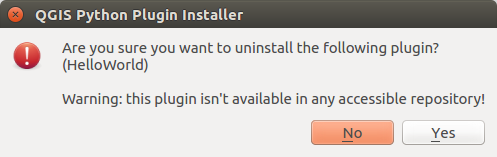
\includegraphics[width=0.5\textwidth]{uninstall_warning.png}
\vspace*{-0.64em}
\caption[La désinstallation d'un plugin personnel efface toutes les données relatives à celui-ci.]{La désinstallation d'un plugin personnel efface toutes les données relatives à celui-ci.\\
Cette opération est \textbf{irréversible} !}
\label{uninstall}
\end{figure}
\vspace*{-1em}


\underline{\smash{Rappel}}: 

Les plugins installés se trouvent dans le dossier : \\
\texttt{C:\textbackslash{}Users\textbackslash{}\textcolor{mygreen}{UserName}\textbackslash{}AppData\textbackslash{}Roaming\textbackslash{}QGIS\textbackslash{}QGIS3\textbackslash{}profiles\textbackslash{}default\textbackslash{}python\textbackslash{}plugins\textbackslash{}}\\
où \textcolor{mygreen}{UserName} est son nom d'utilisateur. 




%%%%%%%%%%%%%%%%%%%%%%%%%%%%%%%%%%%%%%%%
\subsection{Installation des outils}
\label{InstallationDesOutils}
%%%%%%%%%%%%%%%%%%%%%%%%%%%%%%%%%%%%%%%%

Afin de créer de nouveaux plugins QGIS, il est naturellement nécessaire de posséder QGIS (\url{https://qgis.org/download/}) qui comprend notamment QT Designer, permettant ainsi la création simplifiée d'interfaces graphiques pour les plugins. \vspace*{0.2em}

Mais il faut aussi installer \textbf{deux extensions} (plugins) \textbf{supplémentaires} depuis le menu \og{}Extension\fg{} >{} \og{}Installer / Gérer les extensions\fg{} (fig.\,\ref{extensions}) : \vspace*{0.2em}

\begin{itemize}\itemsep0.2em
\renewcommand\labelitemi{\---}
\item \og{}\textbf{Plugin Builder 3}\fg{} (\url{https://plugins.qgis.org/plugins/pluginbuilder3}) qui permet la création du squelette de base pour un plugin (fichiers, structure des dossiers)
\item \og{}\textbf{Plugin Reloader}\fg{} (\url{https://plugins.qgis.org/plugins/plugin_reloader} version min.=0.10) qui permet de recharger les modifications effectuées sur un plugin sans devoir redémarrer QGIS.


\vspace*{-0.2em}
\begin{figure}[H]
	\centering
    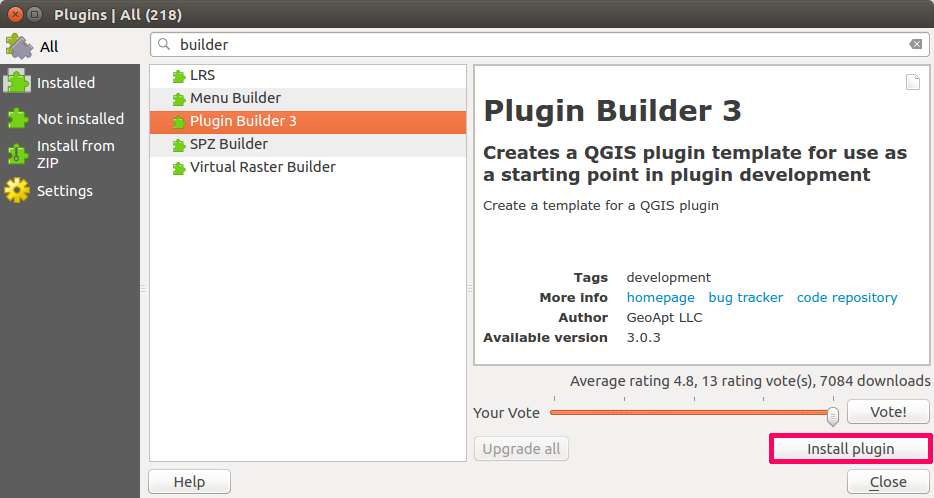
\includegraphics[width=0.8\textwidth]{plugin_builder_install.png}
    \vspace*{-0.4em}
	\caption{Recherche et installation du \og{}Plugin builder 3\fg{}}
    \label{extensions}
\end{figure}


\iffalse

\includegraphics[scale=1]{warningt.png} \underline{\smash{Attention}}: pour installer \og{}Plugin Reloader\fg{}, il est nécessaire de cocher la case "\textbf{Afficher les extensions expérimentales}" dans l'onglet "Paramètres" de la fenêtre de gestion des extensions (fig.\,\ref{experimental}).
\fi
\end{itemize} 
\vspace{1em}

\iffalse
\begin{figure}[H]
	\centering
    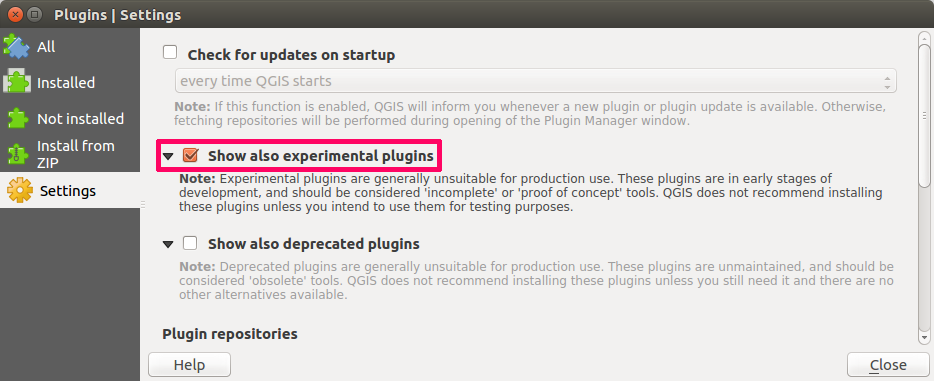
\includegraphics[width=0.8\textwidth]{experimental_flag.png}
	\caption[Sélectionner \og{}Afficher les extensions expérimentales\fg{} pour trouver \og{}Plugin reloader\fg{}.]{Vérifier que la case \og{}Afficher les extensions expérimentales\fg{} soit bien cochée avant de rechercher \og{}Plugin Reloader\fg{}!}
    \label{experimental}
\end{figure}
\fi

\underline{\smash{Résultat}}: après ces opérations, deux nouvelles entrées ont fait leur apparition dans le menu \og{}Extension\fg{} de QGIS ainsi que deux nouveaux boutons dans la barre d'outils principale (fig.\,\ref{fig3}).


\begin{figure}[H]
    \centering
    \begin{subfigure}[t]{0.2\textwidth}
		\centering
        
\includegraphics[width=2em]{pluginbuilder.png}
\caption{Plugin builder}\label{fig3:builder}
    \end{subfigure}%
    ~
    \begin{subfigure}[t]{0.2\textwidth}
        \centering
        
\includegraphics[width=2em]{reload.png}
        \caption{Plugin reloader}\label{fig3:reloader}
    \end{subfigure}
    \caption{Les deux nouveaux boutons apparus dans la barre d'outils principale de QGIS.}
    \label{fig3}
\end{figure}




%%%%%%%%%%%%%%%%%%%%%%%%%%%%%%%%%%%%%%%%
\subsection{Exercice de création d'un plugin}
\label{CreationPlugin}
%%%%%%%%%%%%%%%%%%%%%%%%%%%%%%%%%%%%%%%%
\subsubsection{Contexte}
Cet exercice présente les différentes étapes de création d'un plugin QGIS. Le plugin QGIS alors créé permettra de sélectionner, par l'intermédiaire d'une interface graphique, une des couches ouvertes dans le projet QGIS et d'afficher quelques informations relatives à celle-ci (comme par exemple : le type de couche, le type de géométrie si la couche est de type vectorielle, le système de coordonnées, l'unité du système de coordonnées, etc.). 


\subsubsection{Données}
N'importe quel jeu de données peut être utilisé. Toutefois, afin de pouvoir tester le plugin, il est préférable d'avoir des jeux de données de types différents (raster, vecteur; points, polylignes, polygones). 
Pour ce faire on va à nouveau utiliser des données d'OpenStreetMap : 
%\vspace*{-0.4em}
\begin{center}

\includegraphics[width=1.64cm]{osm.png}\\
\url{http://download.geofabrik.de} 
\end{center}
\vspace*{0.4em}





\newpage{}
\subsubsection{Marche à suivre \--- structure du plugin}
Dans un premier temps, il s'agit de créer la structure des dossiers et fichiers du plugin à l'aide du \og{}Plugin Builder\fg{}. Ensuite, l'interface graphique est modifiée et le code Python correspondant est inséré. 


\begin{enumerate}\itemsep0.4em
\item \textbf{Créer} la structure des dossiers et fichiers à partir du menu \og{}Extension > Plugin Builder > Plugin Builder\fg{} ou du bouton correspondant ( 
\includegraphics[width=1em]{pluginbuilder.png} ) dans la barre d'outils : 

\vspace*{-1em}
\hspace*{-8em}
\begin{minipage}[t]{0.9\paperwidth}
\begin{figure}[H]
    \centering
    \begin{subfigure}[t]{0.32\textwidth}
		\centering
        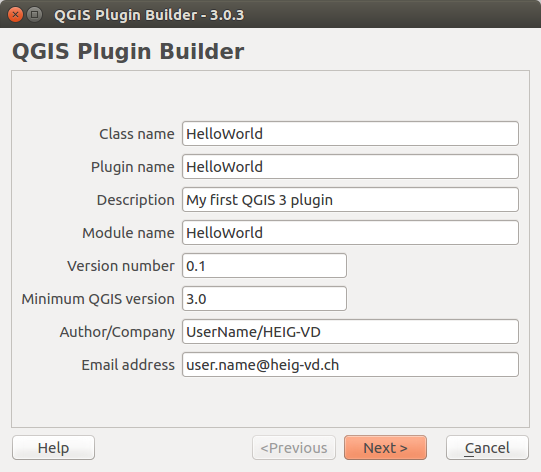
\includegraphics[width=1\textwidth]{pluginbuilder3_1.png}
		\caption{1/6}\label{pluginbuilder:1}
    \end{subfigure}%
    ~
    \begin{subfigure}[t]{0.32\textwidth}
        \centering
        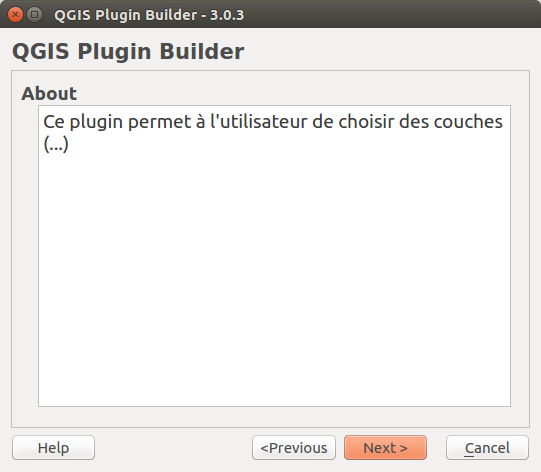
\includegraphics[width=1\textwidth]{pluginbuilder3_2.png}
        \caption{2/6}\label{pluginbuilder:2}
    \end{subfigure}
    ~
    \begin{subfigure}[t]{0.32\textwidth}
        \centering
        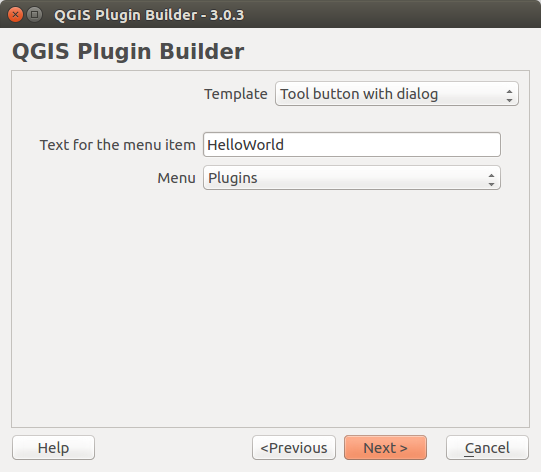
\includegraphics[width=1\textwidth]{pluginbuilder3_3.png}
        \caption{3/6}\label{pluginbuilder:3}
    \end{subfigure}
    \begin{subfigure}[t]{0.32\textwidth}
		\centering
        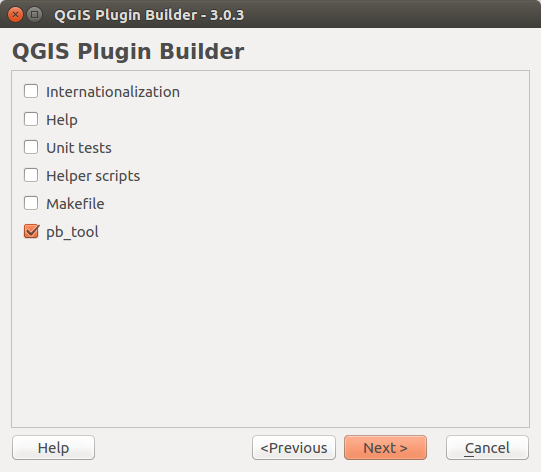
\includegraphics[width=1\textwidth]{pluginbuilder3_4.png}
		\caption{4/6}\label{pluginbuilder:4}
    \end{subfigure}%
    ~
    \begin{subfigure}[t]{0.32\textwidth}
        \centering
        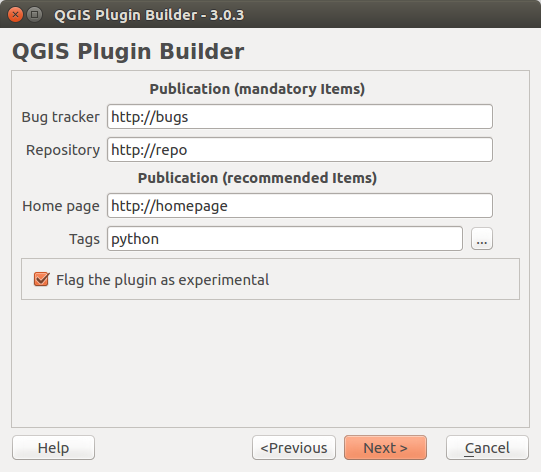
\includegraphics[width=1\textwidth]{pluginbuilder3_5.png}
        \caption{5/6}\label{pluginbuilder:5}
    \end{subfigure}
    ~
    \begin{subfigure}[t]{0.32\textwidth}
        \centering
        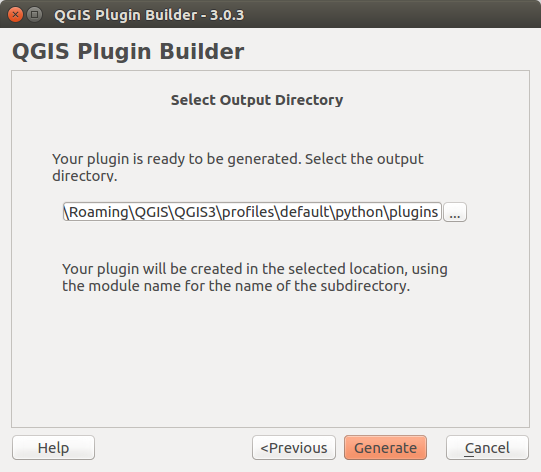
\includegraphics[width=1\textwidth]{pluginbuilder3_6.png}
        \caption{6/6}\label{pluginbuilder:6}
    \end{subfigure}
    \caption[Les 6 étapes de création d'un plugin à l'aide de \og{}Plugin Builder\fg{} dans QGIS.]{Les 6 étapes de création d'un plugin à l'aide de \og{}Plugin Builder\fg{} dans QGIS. \\
    À la dernière étape, au lieu du point affiché, prendre bien soin d'insérer le \textbf{chemin complet} vers le répertoire du plugin : \texttt{C:\textbackslash{}Users\textbackslash{}\textcolor{mygreen}{UserName}\textbackslash{}AppData\textbackslash{}Roaming\textbackslash{}QGIS\textbackslash{}QGIS3\textbackslash{}profiles\textbackslash{}default\textbackslash{}python\textbackslash{}plugins\textbackslash{}}  où \textcolor{mygreen}{UserName} est son nom d'utilisateur.}
    \label{pluginbuilder}
\end{figure}
\end{minipage}
\vspace*{-1em}



$\Rightarrow$ \underline{\smash{Résultat}}: la structure des dossiers et fichiers du plugin a été créée :
\vspace*{-2em}
\begin{center}
\begin{minipage}[t]{0.96\textwidth}
\begin{minted}[frame=single,
  escapeinside=||,
  mathescape,
  linenos,
  numbersep=5pt,
  fontsize=\footnotesize,
  framesep=1mm]{doscon}
C:\Users\UserName\AppData\Roaming\QGIS\QGIS3\profiles\default\python\plugins> tree helloworld/
helloworld/
├── [1.4K]  HelloWorld_dialog_base.ui
├── [1.9K]  HelloWorld_dialog.py
├── [6.5K]  HelloWorld.py
├── [1.0K]  icon.png
├── [1.5K]  __init__.py
├── [ 954]  metadata.txt
├── [2.8K]  pb_tool.cfg
├── [1.8K]  README.html
├── [ 923]  README.txt
└── [ 105]  resources.qrc
\end{minted}
\end{minipage}
\end{center}





\newpage{}

\item Par l'intermédiaire d'une invite de commandes "OSGeo4W Shell" ("menu démarrer > OSGeo4W Shell", il ne faut pas utiliser l'invite de commande de base de Windows) : exécuter au préalable ces deux commandes :
\vspace*{-1em}
\begin{center}
\begin{minipage}[t]{0.92\textwidth}
\begin{minted}[frame=single,
  escapeinside=||,
  mathescape,
  linenos,
  numbersep=5pt,
  fontsize=\footnotesize,
  framesep=1mm]{doscon}
C:\>
py3_env
qt5_env
\end{minted}
\end{minipage}
\end{center}
\vspace*{1em}

Toujours depuis le shell OSGeo4W, se rendre ensuite dans le dossier du plugin et y \textbf{générer} le fichier Python \texttt{resources.py} à partir du fichier \texttt{resources.qrc} grâce à la commande suivante : 
\vspace*{-1em}
\begin{center}
\begin{minipage}[t]{0.92\textwidth}
\begin{minted}[frame=single,
  escapeinside=||,
  mathescape,
  linenos,
  numbersep=5pt,
  fontsize=\footnotesize,
  framesep=1mm]{doscon}
C:\Users\UserName\AppData\Roaming\QGIS\QGIS3\profiles\default\python\plugins\helloworld>
pyrcc5 -o resources.py resources.qrc
\end{minted}
\end{minipage}
\end{center}
\vspace*{1em}






$\Rightarrow$ \underline{\smash{Résultat}}: un nouveau fichier (\og{}\texttt{resources.py}\fg{}) a été créé dans le dossier du plugin. Celui-ci contient la traduction en Python du fichier \og{}\texttt{resources.qrc}\fg{}; un document \texttt{xml} qui contient les liens vers les ressources extérieures (comme par exemple l'icône du plugin). 

\iffalse
\underline{\smash{Remarque}}: Il est également possible de compiler le fichier \og{}resources.qrc\fg{} à l'aide d'OSGeo4W Shell, un fichier \texttt{BAT} du logiciel QGIS. Pour cela: \textbf{lancer} OSGeo4W Shell, se rendre dans le dossier du plugin à l'aide de la commande \og{}\texttt{cd}\fg{} et y exécuter la commande suivante:
\vspace*{-1em}
\begin{center}
\begin{minipage}[t]{0.92\textwidth}
\begin{minted}[frame=single,
  escapeinside=||,
  mathescape,
  linenos,
  numbersep=5pt,
  fontsize=\footnotesize,
  framesep=1mm]{doscon}
C:\Users\UserName\AppData\Roaming\QGIS\QGIS3\profiles\default\python\plugins\helloworld>
pyrcc5 -o resources.py resources.qrc
\end{minted}
\end{minipage}
\end{center}
\vspace*{1em}
\fi



\item À ce stade il est nécessaire de \textbf{redémarrer} QGIS pour qu'il prenne en compte le nouveau plugin.

\begin{figure}[H]
  	\centering		
	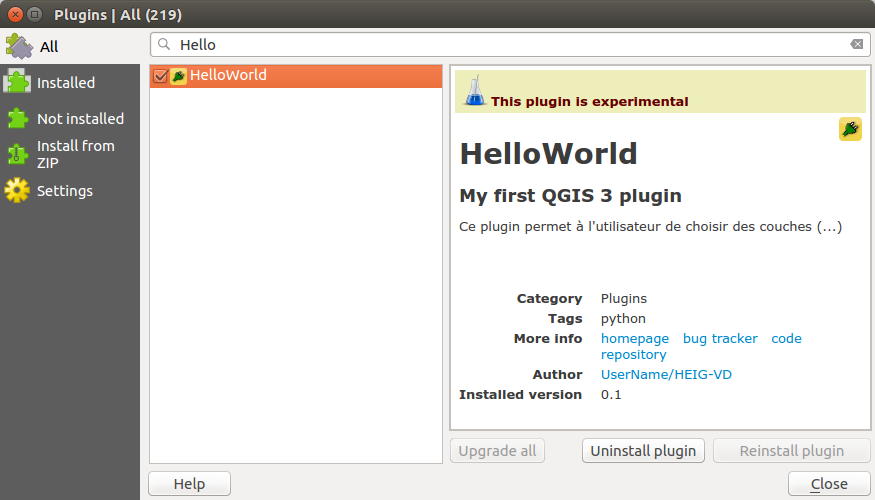
\includegraphics[width=0.8\textwidth]{hello2018_plugin.png}
	\caption[Le plugin créé est installé; QGIS l'a bien reconnu au redémarrage !]{Le plugin créé est installé; QGIS l'a bien reconnu au redémarrage !\\
	Le plugin se trouve dans le menu \og{}Extension > Installer / Gérer les extensions\fg{} > onglet \og{}Installées\fg{} ou \og{}Toutes\fg{}.}
	\label{hello2018}
\end{figure}


\item \textbf{Ouvrir} le plugin. Il est maintenant directement exécutable depuis le menu :\\
\og{}Extension > HelloWorld > 
\includegraphics[width=0.76em]{hello2018_icon.png} HelloWorld\fg{} ou à l'aide du bouton correspndant ( 
\includegraphics[width=1em]{hello2018_icon.png} ) dans la barre d'outils.


$\Rightarrow$ \underline{\smash{Résultat}}: pour l'instant, l'interface graphique du plugin n'est composée que de 2 boutons (fig.\,\ref{plugin_buttons}):

\vspace*{-0.8em}
\begin{figure}[H]
    \centering
    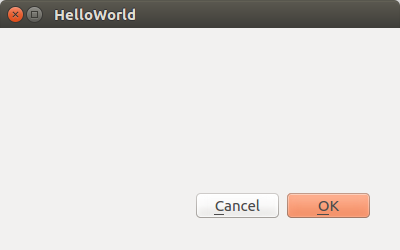
\includegraphics[width=0.44\textwidth]{hello2018.png}
    \vspace*{-0.8em}
    \caption{La fenêtre du nouveau plugin !}
    \label{plugin_buttons}
\end{figure}
\vspace*{-0.64em}

Pour ajouter de nouveaux éléments à cette fenêtre, il faut travailler sur l'interface graphique du plugin à l'aide de Qt Designer. C'est ce point qui est abordé dans la prochaine section.

\end{enumerate}




\section*{Notes}
\hrulefill
\vspace*{1.6em}

\hrulefill
\vspace*{1.6em}

\hrulefill
\vspace*{1.6em}

\hrulefill
\vspace*{1.6em}

\hrulefill
\vspace*{1.6em}

\hrulefill
\vspace*{1.6em}

\hrulefill
\vspace*{1.6em}

\hrulefill
\vspace*{1.6em}

\hrulefill
\vspace*{1.6em}

\hrulefill
\vspace*{1.6em}

\hrulefill
\vspace*{1.6em}

\hrulefill
\vspace*{1.6em}

\hrulefill
\vspace*{1.6em}
















\newpage{}
\vspace*{-3.2em}
\subsubsection{Marche à suivre \--- interface graphique du plugin}
Il s'agit à présent de modifier l'interface graphique grâce au logiciel \og{}\textbf{Qt Designer}\fg{}. \\

\vspace*{-0.4em}

\includegraphics[scale=1]{warningt.png} \underline{\smash{Attention}}: afin de pouvoir constater les modifications effectuées sur l'interface graphique, il est nécessaire de \textbf{recharger} le plugin. Ceci se réalise en redémarrant QGIS ou en utilisant le \og{}Plugin Reloader\fg{}. 




\begin{enumerate}\itemsep0.4em
\item Par l'intermédiaire de l'explorateur Windows : \textbf{se rendre} dans le dossier du plugin :\\
\texttt{C:\textbackslash{}Users\textbackslash{}\textcolor{mygreen}{UserName}\textbackslash{}AppData\textbackslash{}Roaming\textbackslash{}QGIS\textbackslash{}QGIS3\textbackslash{}profiles\textbackslash{}default\textbackslash{}python\textbackslash{}plugins}\\
où \textcolor{mygreen}{UserName} est son nom d'utilisateur.


\item \textbf{Ouvrir} le fichier ayant l'extension \og{}\texttt{.ui}\fg{} avec le logiciel \og{}Qt Designer\fg{}: pour cela réaliser un clic droit sur le fichier et choisir \og{}Ouvrir avec...\fg{} puis sélectionner \og{}Qt Designer\fg{} dans la liste des programmes. S'il ne s'y trouve pas, choisir alors \og{}Autre\fg{} et naviguer jusqu'au fichier exécutable du programme sous \texttt{C:\textbackslash{}Programmes\textbackslash{}QGIS\_\textcolor{green}{<VERSION>}\textbackslash{}bin\textbackslash{}qgis-designer.bat} (il serait aussi possible de démarrer une version indépendante du logiciel si elle était installée). Remplacer \textcolor{green}{<VERSION>} par le numéro de version de QGIS, par exemple 3.2.

\underline{\smash{Remarque}}: \vspace*{0.4em}
\begin{itemize}\itemsep0.4em
\renewcommand\labelitemi{\---}
\item On peut durablement choisir d'ouvrir les fichiers de type \og{}\texttt{.ui}\fg{} par un clic droit sur un tel fichier et en se rendant sous \og{}Propriétés\fg{} > onglet \og{}Général\fg{} > bouton \og{}Modifier\fg{} pour finalement choisir le programme adéquat dans l'explorateur avant d'enregistrer les nouvelles propriétés du fichier. Un double-clic sur un fichier \og{}\texttt{.ui}\fg{} fait alors directement appel à \og{}Qt Designer\fg{}.


\item L'interface graphique est contenue dans ce fichier \og{}\texttt{.ui}\fg{} sous la forme de code \texttt{XML}. Les différentes balises qu'il contient correspondent aux différents éléments de l'interface graphique:

\vspace*{-1.2em}
\begin{center}
\begin{minipage}[t]{0.9\textwidth}
\begin{minted}[frame=single,
  escapeinside=||,
  mathescape,
  linenos,
  numbersep=5pt,
  fontsize=\scriptsize,
  framesep=1mm]{xml}
<ui version="4.0" >
 <class>HelloWorldDialogBase</class>
 <widget class="QDialog" name="HelloWorldDialogBase" >
  <property name="geometry" >
   <rect>
    <x>0</x>
    <y>0</y>
    <width>400</width>
    <height>300</height>
   </rect>
  </property>
  <property name="windowTitle" >
   <string>HelloWorld</string>
  </property>
  <widget class="QDialogButtonBox" name="button_box" >
   <property name="geometry" >
    <rect>
     <x>30</x>
     <y>240</y>
     <width>341</width>
     <height>32</height>
    </rect>
   </property>
   <property name="orientation" >
    <enum>Qt::Horizontal</enum>
   </property>
   <property name="standardButtons" >
    <set>QDialogButtonBox::Cancel|QDialogButtonBox::Ok</set>
   </property>
  </widget>
 </widget>
(...)
</ui>
\end{minted}
\end{minipage}
\end{center}
\vspace*{1em} 

\underline{\smash{Remarque}}: chaque bouton, chaque étiquette, chaque liste, etc. est un \emph{\textbf{widget}} dans le code \texttt{XML}. 
\end{itemize}



\newpage{}
\item À l'aide des fenêtres \og{}Boîte de widgets\fg{} et \og{}Éditeur de propriétés\fg{} : \textbf{ajouter} de nouveaux éléments dans l'interface graphique du plugin (fig.\,\ref{qt}) et en parallèle, \textbf{visualiser} le résultat sous QGIS. 

\underline{\smash{Remarque}}: 
\begin{itemize}\itemsep0.2em
\renewcommand\labelitemi{\---}
\item Pour ouvrir les fenêtres \og{}Boîte de widget\fg{} et \og{}Éditeur de propriétés\fg{} si elles ne le sont pas déjà dans \og{}Qt Designer\fg{} : utiliser le menu \og{}Affichage\fg{} du logiciel. 
\item Pour visualiser les modifications de l'interface graphique dans QGIS : utiliser le \og{}Plugin Reloader\fg{} dans le menu \og{}Extension\fg{} > \og{}Plugin Reloader\fg{} ou avec le bouton correspondant : 
\begin{center}

\includegraphics[width=2em]{reload.png}
\end{center}

\end{itemize}

\begin{figure}[H]
    \centering
    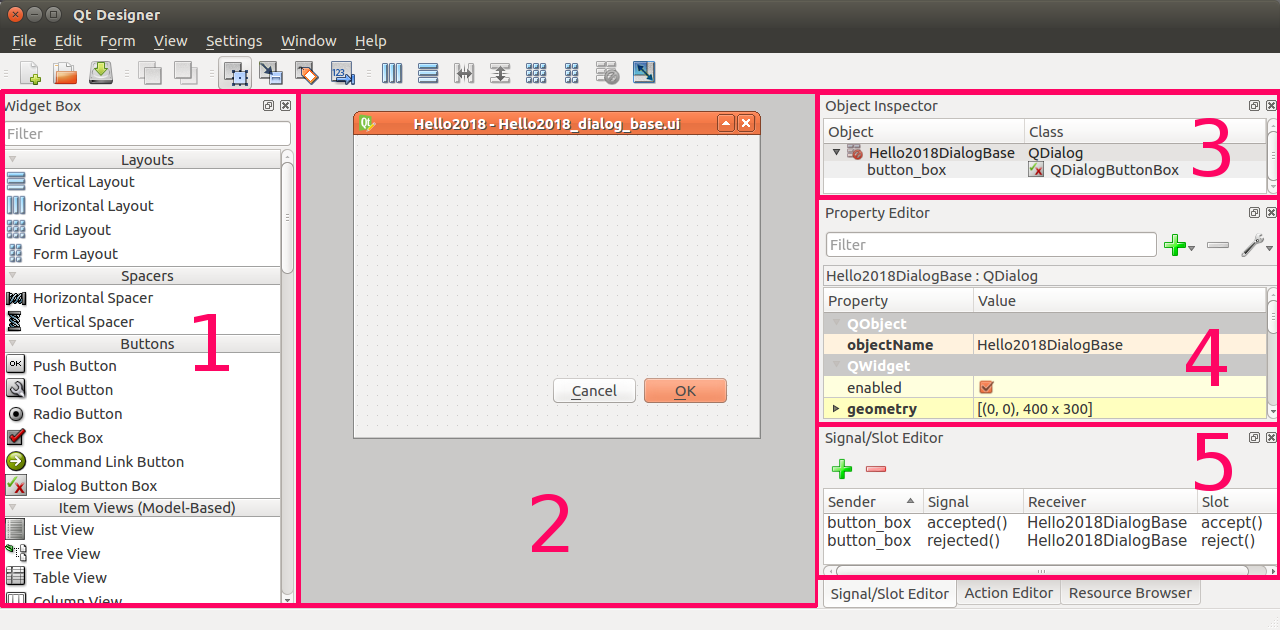
\includegraphics[width=1\textwidth]{qtdesigner5w2.png}
    \vspace*{-1.44em}
    \caption[Fenêtre principale de Qt Designer.]{Fenêtre principale de Qt Designer.\\ 1: Boîte à widgets. 2: Fenêtre de dessin. 3: Inspecteur d'objets. 4: Éditeur de propriétés. 5: Trois onglets; a) éditeur de signaux/slots, b) éditeur d'actions, c) explorateur de ressources.}
    \label{qt}
\end{figure}




\includegraphics[scale=1]{warningt.png} \underline{\smash{Attention}}: ne pas oublier de \textbf{régulièrement enregistrer} les modifications de l'interface graphique (menu \og{}Fichier > Enregistrer \fg{} de \og{}Qt Designer\fg{}). 


\section*{Notes}
\hrulefill
\vspace*{1.6em}

\hrulefill
\vspace*{1.6em}

\hrulefill
\vspace*{1.6em}

\hrulefill
\vspace*{1.6em}










\newpage{}
Les éléments à \textbf{ajouter} dans l'interface graphique sont les suivants:

\begin{itemize}\itemsep0.2em
\renewcommand\labelitemi{\---}
\item Un titre grâce à un \og{}Label\fg{} de la section \og Display Widgets \fg{}. Le titre est à centrer et mettre en taille de police 12.
\item Une liste déroulante avec une \og Combo Box \fg{}  dans la section \og Input Widgets \fg{}.
\item Un bouton avec \og Push Button \fg{} dans la section \og Buttons \fg{} qui s'appelle \og Sélectionner \fg{}.
\end{itemize}

Le rendu final doit ressembler à la figure \ref{ig}.


\vspace*{-0.4em}
\begin{figure}[H]
    \centering
    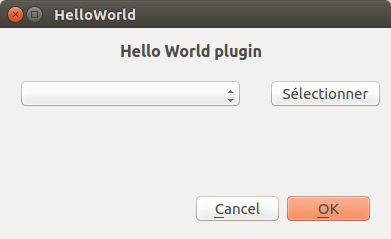
\includegraphics[width=0.44\textwidth]{plugin_layout.png}
    \vspace*{-0.8em}
    \caption[Interface graphique du plugin]{Interface graphique du plugin QGIS construite dans Qt Designer.}
    \label{ig}
\end{figure}



\underline{\smash{Remarque}}: la liste déroulante est pour l'instant vide et sera remplie des différentes couches présentes dans le projet QGIS dans le cadre du prochain chapitre. 


\end{enumerate}




\subsubsection{Marche à suivre \--- code Python du plugin}
A présent, l'interface graphique possède plusieurs éléments d'interaction, mais ceux-ci ne sont actuellement pas utilisables. Afin de pouvoir créer l'interaction avec les utilisateurs, il est nécessaire de modifier le code Python qui se trouve dans le fichier Python principal (ici : \og{}HelloWorld.py\fg{}), plus précisément dans la fonction \texttt{run()} de ce fichier.

\paragraph*{Introduction}

\begin{enumerate}\itemsep0.4em
\item Pour \textbf{vérifier} que le plugin réponde bien : \textbf{ajouter} tout d'abord une fonction \og{}\texttt{print()}\fg{} dans la condition \og \texttt{if} \fg{} avec l'éditeur de votre choix (par exemple: Notepad++) :

\vspace*{-2em}
\begin{center}
\begin{minipage}[t]{0.98\textwidth}
\begin{minted}[frame=single,
  escapeinside=||,
  mathescape,
  %bgcolor=lbcolor,
  linenos,
  numbersep=5pt,
  fontsize=\small,
  framesep=1mm]{python3}
def run(self):
    """Run method that performs all the real work"""
    # show the dialog
    self.dlg.show()
    # Run the dialog event loop
    result = self.dlg.exec_()
    # See if OK was pressed
    if result:
        # Do something useful here - delete the line containing pass and
        # substitute with your code.
        print("Button OK of the plugin is successfully pushed!")
        pass
\end{minted}
\end{minipage}
\end{center}
\vspace*{0.4em}

\underline{\smash{Remarque}}: en Python, les fonctions sont définies avec le mot-clé \og \texttt{def} \fg{} suivi du nom que l'on souhaite donner à sa nouvelle fonction.

\vspace*{0.4em}
\item Depuis QGIS : \textbf{recharger} le plugin à l'aide du \og{}Plugin Reloader\fg{}, \textbf{ouvrir} la console Python et tester le fonctionnement du plugin





\newpage{}
$\Rightarrow$ \underline{\smash{Résultat}}: le texte est inscrit dans la console Python lorsque le bouton \og OK \fg{} est appuyé (fig.\,\ref{resplug})):


\begin{figure}[H]
    \centering
    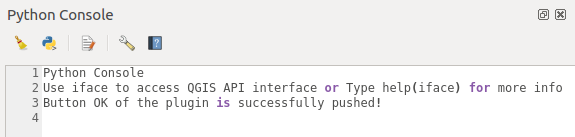
\includegraphics[width=0.64\textwidth]{plugin_first_result.png}
    \vspace*{-0.8em}
    \caption[Affichage du résultat du plugin dans la console Python.]{Affichage du résultat du plugin dans la console Python.}
    \label{resplug}
\end{figure}


\underline{\smash{Remarque}}: le mot \og \texttt{is} \fg{} est différent des autres mots, car celui-ci est un mot-clé de Python. Toutefois, comme il est considéré comme une chaîne de caractères dans ce cas-ci, il peut sans problème être utilisé. 

\paragraph*{Affichage des couches dans la liste déroulante de l'interface graphique}


\item \textbf{Ajouter} une nouvelle fonction (exemple de nom : \og{}\texttt{loadActiveLayers}\fg{}) dans le fichier Python principal (ici : \og{}HelloWorld.py\fg{}) et appeler cette nouvelle fonction depuis la fonction \og{}\texttt{run()}\fg{} :
\vspace*{-1em}
\begin{center}
\begin{minipage}[t]{0.28\textwidth}
\begin{minted}[frame=single,
  escapeinside=||,
  mathescape,
  %bgcolor=lbcolor,
  linenos,
  numbersep=5pt,
  fontsize=\small,
  framesep=1mm]{python3}
self.loadActiveLayers()
\end{minted}
\end{minipage}
\end{center}
\vspace*{1em}




 
\item \textbf{Récupérer} les couches qui ont été préalablement chargées dans QGIS avec les deux lignes de code suivantes : 
\vspace*{-1.64em}
\begin{center}
\begin{minipage}[t]{0.36\textwidth}
\begin{minted}[frame=single,
  escapeinside=||,
  mathescape,
  %bgcolor=lbcolor,
  linenos,
  numbersep=5pt,
  fontsize=\small,
  framesep=1mm]{python3}
canvas = iface.mapCanvas()
activeLayers = canvas.layers()
\end{minted}
\end{minipage}
\end{center}
\vspace*{1em}




\includegraphics[scale=1]{warningt.png} \underline{\smash{Attention}}: afin de pouvoir utiliser \og{}\texttt{iface}\fg{}, il est nécessaire d'ajouter l'import suivant \textbf{en haut} du fichier Python principal :
\vspace*{-1em}
\begin{center}
\begin{minipage}[t]{0.30\textwidth}
\begin{minted}[frame=single,
  escapeinside=||,
  mathescape,
  %bgcolor=lbcolor,
  linenos,
  numbersep=5pt,
  fontsize=\small,
  framesep=1mm]{python3}
from qgis.utils import *
\end{minted}
\end{minipage}
\end{center}
\vspace*{1em}

\underline{\smash{Remarque}}: 
\begin{itemize}\itemsep0.2em
\renewcommand\labelitemi{\---}
\item \og{}\texttt{iface}\fg{} est un objet de la classe \og{}\texttt{QgsInterface}\fg{} qui permet d'accéder au canevas de carte, aux menus, aux barres d'outils, etc. tandis que la fonction \og{}\texttt{mapCanvas()}\fg{} retourne un objet de type \og{}\texttt{QgsMapCanvas}\fg{}. 
\item La deuxième ligne de code permet de récupérer toutes les couches de l'objet \og{}\texttt{canvas}\fg{} présentes dans le projet QGIS actuellement ouvert. \og{}\texttt{activeLayers}\fg{} est une variable qui contient donc une liste de toutes les couches présentes. 
\end{itemize}



\item \textbf{Récupérer} et \textbf{afficher} le nom de chaque couche à partir de la variable  \og{}\texttt{activeLayers}\fg{}  précédemment définie et par l'intermédiaire d'une boucle : 
\vspace*{-1em}
\begin{center}
\begin{minipage}[t]{0.32\textwidth}
\begin{minted}[frame=single,
  escapeinside=||,
  mathescape,
  %bgcolor=lbcolor,
  linenos,
  numbersep=5pt,
  fontsize=\small,
  framesep=1mm]{python3}
for layer in activeLayers:
    # corps de la boucle
\end{minted}
\end{minipage}
\end{center}
\vspace*{1em}



\item En utilisant la méthode \og{}\texttt{name()}\fg{} dans la boucle précédemment créée, il est possible de \textbf{récupérer} le nom de chaque couche : 
\vspace*{-1.64em}
\begin{center}
\begin{minipage}[t]{0.30\textwidth}
\begin{minted}[frame=single,
  escapeinside=||,
  mathescape,
  %bgcolor=lbcolor,
  linenos,
  numbersep=5pt,
  fontsize=\small,
  framesep=1mm]{python3}
layerName = layer.name()
\end{minted}
\end{minipage}
\end{center}
\vspace*{1em}

\underline{\smash{Remarque}}: \og{}\texttt{layer}\fg{} représente chacune des couches à tour de rôle. Ainsi, au premier tour de la boucle, la variable \og{}\texttt{layer}\fg{} contient les données de la première couche. Au deuxième tour, de la deuxième couche, etc. 

\item Toujours dans la boucle : \textbf{récupérer} à présent le type de fichier de chaque couche avec la méthode \og{}\texttt{type()}\fg{}

\underline{\smash{Remarque}}: La méthode \og{}\texttt{type()}\fg{} retourne une valeur de \og{}\texttt{0}\fg{} pour une couche vectorielle et une valeur de \og{}\texttt{1}\fg{} pour une couche de type raster.  


\item Toujours au sein de la boucle : \textbf{créer} une nouvelle variable (par exemple de nom : \og{}\texttt{layerType}\fg{}) et la définir de la manière suivante : 

\begin{itemize}\itemsep0.2em
\renewcommand\labelitemi{\---}
\item Si la méthode \og{}\texttt{type()}\fg{} retourne \og{}\texttt{0}\fg{} $\Rightarrow$ la variable \og{}\texttt{layerType}\fg{} = "\texttt{vecteur}" 
\item Si la méthode \og{}\texttt{type()}\fg{} retourne \og{}\texttt{1}\fg{} $\Rightarrow$ la variable \og{}\texttt{layerType}\fg{} = "\texttt{raster}" 
\end{itemize}

\includegraphics[scale=1]{tip_l.png} \underline{\smash{Astuce}}: utiliser une condition (\texttt{if: ... elif: ... else: ...}). 

\includegraphics[scale=1]{warningt.png} \underline{\smash{Attention}}: il est nécessaire de convertir le résultat de la méthode \og{}\texttt{type()}\fg{} en chaîne de caractères (\og{}\texttt{string}\fg{}) à l'aide de la fonction \og{}\texttt{str()}\fg{}. 


\item Toujours dans la boucle : \textbf{ajouter} la ligne de code suivante afin de pouvoir ajouter le nom et le type de chacune des couches dans la liste déroulante (ici : \og{}\texttt{comboBox}\fg{}):
\vspace*{-1em}
\begin{center}
\begin{minipage}[t]{0.44\textwidth}
\begin{minted}[frame=single,
  escapeinside=||,
  mathescape,
  %bgcolor=lbcolor,
  linenos,
  numbersep=5pt,
  fontsize=\small,
  framesep=1mm]{python3}
self.dlg.comboBox.addItem(layerName)
\end{minted}
\end{minipage}
\end{center}
\vspace*{1em}

\includegraphics[scale=1]{warningt.png} \underline{\smash{Attention}}: \og{}\texttt{comboBox}\fg{} fait référence au nom de la liste déroulante qui a été définie dans \og{}Qt Designer\fg{} dans le fichier d'extension \og{}\texttt{ui}\fg{} (\texttt{HelloWorld\_dialog\_base.ui}) : 


$\Rightarrow$ \underline{\smash{Exemple du résultat attendu}}: 

\begin{figure}[H]
    \centering
    \includegraphics[width=0.44\textwidth]{layer_type.png}
    \vspace*{-0.2em}
    \caption[Sélecteur de couches du plugin QGIS]{Sélecteur de couches du plugin QGIS. Le type de couche doit figurer entre parenthèses après son nom.}
    \label{selecteur}
\end{figure}


\item \textbf{Tester} le plugin dans QGIS !

\includegraphics[scale=1]{warningt.png} \underline{\smash{Attention}}: ne pas oublier de \textbf{recharger} les modifications avec le \og{}Plugin Reloader\fg{}. 







\newpage{}
\vspace*{-2.4em}
\includegraphics[scale=1]{warningt.png} \underline{\smash{Problème}}: en exécutant plusieurs fois la fonction de chargement des couches (ici :\\\og{}\texttt{loadActiveLayers()}\fg{}), les différentes couches s'ajoutent à chaque fois; on les retrouve donc à double, à triple, etc. :
\vspace*{-0.4em} 
\begin{figure}[H]
    \centering
    \includegraphics[width=0.44\textwidth]{layer_type_issue.png}
    \vspace*{-0.2em}
    \caption[Problème dans le sélecteur de couches]{Problème dans le sélecteur de couches du plugin; les couches d'additionnent à chaque fois qu'on recharge le plugin !}
    \label{selecterissue}
\end{figure}

Pour y remédier, il suffit d'effectuer un \textbf{nettoyage} de la liste déroulante au \textbf{début} de la fonction (ici : \og{}\texttt{loadActiveLayers()}\fg{}) à l'aide de la méthode \og{} \texttt{clear()} \fg{} :
\vspace*{-1em}
\begin{center}
\begin{minipage}[t]{0.30\textwidth}
\begin{minted}[frame=single,
  escapeinside=||,
  mathescape,
  %bgcolor=lbcolor,
  linenos,
  numbersep=5pt,
  fontsize=\small,
  framesep=1mm]{python3}
self.dlg.comboBox.clear()
\end{minted}
\end{minipage}
\end{center}
\vspace*{0.4em}



\paragraph*{Récupération de la couche sélectionnée par l'utilisateur}

\item Dans le fichier Python principal : \textbf{créer} une nouvelle fonction (exemple de nom : \og{}\texttt{makeSomeStatistics()}\fg{}) qui est appelée lors du clic sur le bouton \og{}Sélectionner\fg{}.

\item \textbf{Récupérer} le clic sur le bouton \og{}Sélectionner\fg{} dans la fonction \og{}\texttt{add\_action()}\fg{} du fichier Python principal : 
\vspace*{-1em}
\begin{center}
\begin{minipage}[t]{0.70\textwidth}
\begin{minted}[frame=single,
  escapeinside=||,
  mathescape,
  %bgcolor=lbcolor,
  linenos,
  numbersep=5pt,
  fontsize=\small,
  framesep=1mm]{python3}
self.dlg.pushButton.clicked.connect(self.makeSomeStatistics)
\end{minted}
\end{minipage}
\end{center}
\vspace*{0.4em}

\includegraphics[scale=1]{warningt.png} \underline{\smash{Attention}}: \og{}\texttt{pushButton}\fg{} fait référence au nom du bouton \og{}Sélectionner\fg{} qui a été défini dans \og{}Qt Designer\fg{} dans le fichier d'extension \og{}\texttt{ui}\fg{} (fig.\,\ref{pushbutton}) : 
\vspace*{-0.4em}
\begin{figure}[H]
    \centering
    \begin{subfigure}[t]{0.44\textwidth}
    \centering
    	\includegraphics[width=1\textwidth]{qtpushbutton.png}
    	\caption{Dans Qt Designer.}
    	\label{pushbutton:qt}
    \end{subfigure}
    ~
    \begin{subfigure}[t]{0.44\textwidth}
    \centering
    		\includegraphics[width=1\textwidth]{push_button.png}
    	\caption{Dans le fichier \texttt{HelloWorld\_dialog\_base.ui}}
    	\label{pushbutton:ui}
    \end{subfigure}
    \vspace*{-0.64em}
    \caption[Nom du bouton \og{}Sélectionner\fg{}]{Nom du bouton \og{}Sélectionner\fg{} qui est utilisé par Python.}
    \label{pushbutton}
\end{figure}

\og{}\texttt{makeSomeStatistics}\fg{} est le nom de la fonction qui est exécutée lorsque le bouton \og{}\texttt{pushButton}\fg{} est cliqué (\og{}\texttt{clicked}\fg{}). 

\item Dans la nouvelle fonction précédemment créée : \textbf{récupérer} la couche sélectionnée par l'utilisateur en récupérant l'index de la couche dans la liste déroulante : 
\vspace*{-1em}
\begin{center}
\begin{minipage}[t]{0.48\textwidth}
\begin{minted}[frame=single,
  escapeinside=||,
  mathescape,
  %bgcolor=lbcolor,
  linenos,
  numbersep=5pt,
  fontsize=\small,
  framesep=1mm]{python3}
index = self.dlg.comboBox.currentIndex()
\end{minted}
\end{minipage}
\end{center}
\vspace*{.8em}

\underline{\smash{Remarque}}: à partir de cet index, il est possible de récupérer l'objet qui a été sélectionné par l'utilisateur : 
\vspace*{-1.64em}
\begin{center}
\begin{minipage}[t]{0.60\textwidth}
\begin{minted}[frame=single,
  escapeinside=||,
  mathescape,
  %bgcolor=lbcolor,
  linenos,
  numbersep=5pt,
  fontsize=\small,
  framesep=1mm]{python3}
canvas = iface.mapCanvas()
selectedLayer = canvas.layers()[index]
print("Couche selectionnee: ", selectedLayer.name())
\end{minted}
\end{minipage}
\end{center}
\vspace*{1em}


$\Rightarrow$ \underline{\smash{Exemple du résultat attendu}}:
\begin{figure}[H]
    \centering
    \includegraphics[width=0.9\textwidth]{clicked.png}
    \vspace*{-0.4em}
    \caption[Affichage en console du nom de la couche par simple clic sur le bouton \og{}Sélectionner\fg{}]{Un clic sur le bouton \og{}Sélectionner\fg{} permet d'afficher le nom de la couche dans la console.}
    \label{res2}
\end{figure}
\vspace*{-1em}

\paragraph*{Affichage de quelques informations relatives à la couche sélectionnée}

\item \textbf{Modifier} l'interface graphique de manière à afficher quelques informations relatives à la couche sélectionnée (fig.\,\ref{qt_labels}): 

\vspace*{-1.8em}
\begin{figure}[H]
    \centering
    \includegraphics[width=0.4\textwidth]{qt_labels.png}
    \vspace*{-0.4em}
    \caption[Ajout de \og{}Labels\fg{} à l'interface graphique]{Dans ce cas-ci, des \og{}Label\fg{} (de la section \og{}Display Widgets\fg{}) ont été utilisés pour les textes déjà écrits (exemple : \og{} Geometry : \fg{}). On viendra ensuite ajouter au contenu de ces labels d'autres informations par l'intermédiaire de code Python.}
    \label{qt_labels}
\end{figure}
\vspace*{-1em}


Voici quelques idées d'informations qui pourraient être affichées : 

\begin{itemize}\itemsep0.2em
\renewcommand\labelitemi{\---}
\item Type de géométrie : ponctuel, linéaire, surfacique
\item Système de coordonnées : par ex. : EPSG:2056
\item Unité de la couche : [mètre] par exemple 
\item Nombre d'objets dans la couche 
\item Noms des différents champs de la table attributaire 
\item étendue géographique de la couche
\item ...
\end{itemize}

\item \textbf{Récupérer} les différentes informations (par exemple : le type de couche, la géométrie de la couche si celle-ci est de type vectoriel, le code EPSG du système de coordonnées, l'unité du système de coordonnées) à l'aide des fonctions respectives (\textbf{s'aider} de la documentation et d'Internet pour trouver les différentes fonctions!), par exemple : 
\vspace*{-0.8em}
\begin{center}
\begin{minipage}[t]{0.40\textwidth}
\begin{minted}[frame=single,
  escapeinside=||,
  mathescape,
  %bgcolor=lbcolor,
  linenos,
  numbersep=5pt,
  fontsize=\small,
  framesep=1mm]{python3}
str(selectedLayer.geometryType())
\end{minted}
\end{minipage}
\end{center}
\vspace*{0.4em}



\underline{\smash{Remarque}}: 
\vspace*{0.4em}
\begin{itemize}\itemsep0.2em
\renewcommand\labelitemi{\---}
\item La fonction \og{}\texttt{str()}\fg{} permet de convertir le résultat qui est de type :
\vspace*{-0.2em}
\begin{center}
\begin{minipage}[t]{0.40\textwidth}
\begin{minted}[frame=single,
  escapeinside=||,
  mathescape,
  %bgcolor=lbcolor,
  linenos,
  numbersep=5pt,
  fontsize=\small,
  framesep=1mm]{python3}
<class 'qgis._core.GeometryType'>
\end{minted}
\end{minipage}
\end{center}
\vspace*{1em}

en chaîne de caractères. \vspace*{0.2em}

\includegraphics[scale=1]{tip_l.png} \underline{\smash{Astuce}}: pour connaître le type d'une variable: utiliser la fonction  \og{}\texttt{type()}\fg{} !






%\newpage{}
\item La fonction \og{}\texttt{geometryType()}\fg{} permet de connaître le type de géométrie si la couche est vectorielle, c'est-à-dire s'il s'agit de données ponctuelles, linéaires ou surfaciques.

\includegraphics[scale=1]{warningt.png} \underline{\smash{Attention}}: si la couche n'est pas vectorielle (ndlr : si la couche est de type raster), le code renvoie une erreur. $\Rightarrow$ dans le code Python, il est donc important de tester (à l'aide de la fonction \og{}\texttt{type()}\fg{} et l'ajout d'une condition) le type de géométrie \textbf{avant} d'appliquer la fonction \og{}\texttt{geometryType()}\fg{} afin de ne pas l'appliquer à une couche de type raster : 
\vspace*{-0.2em}
\begin{center}
\begin{minipage}[t]{0.44\textwidth}
\begin{minted}[frame=single,
  escapeinside=||,
  mathescape,
  %bgcolor=lbcolor,
  linenos,
  numbersep=5pt,
  fontsize=\small,
  framesep=1mm]{python3}
layerType = str(selectedLayer.type())
if layerType == '1':
    geomTxt = 'Raster'
elif layerType == '0':
    geomTxt = 'Vecteur'
else:
    geomTxt = 'Geometrie inconnue!'
\end{minted}
\end{minipage}
\end{center}
\vspace*{1em}
\end{itemize}


\item \textbf{Afficher} ces différentes informations dans l'interface graphique en sélectionnant l'élément graphique en question (exemple : le label xxx) : 
\vspace*{-1em}
\begin{center}
\begin{minipage}[t]{0.4\textwidth}
\begin{minted}[frame=single,
  escapeinside=||,
  mathescape,
  %bgcolor=lbcolor,
  linenos,
  numbersep=5pt,
  fontsize=\small,
  framesep=1mm]{python3}
self.dlg.label_5.setText(geomTxt)
\end{minted}
\end{minipage}
\end{center}


\underline{\smash{Remarque}}:

\begin{itemize}\itemsep0.2em
\renewcommand\labelitemi{\---}
\item \og{}\texttt{label\_5}\fg{} est le nom du label dans le fichier \og{}\texttt{.ui}\fg{}. 
\item La fonction \og{}\texttt{setText()}\fg{} permet d'ajouter du texte au label en question. Le paramètre de la fonction \og{}\texttt{setText()}\fg{} (ndlr : la valeur entre les parenthèses de la fonction ; ici : variable qui a été nommée \og{}\texttt{geomTxt()}\fg{}) est le texte en question. 
\end{itemize}

\includegraphics[scale=1]{warningt.png} \underline{\smash{Attention}}: ne pas oublier d'effectuer un nettoyage du texte de chaque label grâce à la méthode \og{}\texttt{clear()}\fg{} qui est à placer au début de la fonction (ici : \og{}\texttt{makeSomeStatistics}\fg{}) :
\vspace*{-1em}
\begin{center}
\begin{minipage}[t]{0.30\textwidth}
\begin{minted}[frame=single,
  escapeinside=||,
  mathescape,
  %bgcolor=lbcolor,
  linenos,
  numbersep=5pt,
  fontsize=\small,
  framesep=1mm]{python3}
self.dlg.label_5.clear()
\end{minted}
\end{minipage}
\end{center}


\section*{Notes}
\hrulefill
\vspace*{1.6em}

\hrulefill
\vspace*{1.6em}

\hrulefill
\vspace*{1.6em}

\hrulefill
\vspace*{1.6em}

\hrulefill
\vspace*{1.6em}

\hrulefill
\vspace*{1.6em}

\hrulefill
\vspace*{1.6em}

\hrulefill
\vspace*{1.6em}

\hrulefill
\vspace*{1.6em}

\hrulefill
\vspace*{1.6em}

\hrulefill
\vspace*{1.6em}

\hrulefill
\vspace*{1.6em}

\hrulefill
\vspace*{1.6em}

\hrulefill
\vspace*{1.6em}

\hrulefill
\vspace*{1.6em}

\hrulefill
\vspace*{1.6em}

\hrulefill
\vspace*{1.6em}

\hrulefill
\vspace*{1.6em}

\hrulefill
\vspace*{1.6em}







\newpage{}
$\Rightarrow$ \underline{\smash{Exemple du résultat attendu}}:

\vspace*{-0em}
\hspace*{-8em}
\begin{minipage}[t]{0.9\paperwidth}
\begin{figure}[H]
    \centering
    \begin{subfigure}[t]{0.44\textwidth}
		\centering
        \includegraphics[width=1\textwidth]{plugintest1_4.png}
		\caption{Points en WGS84}\label{plugintest:1}
    \end{subfigure}%
    ~
    \begin{subfigure}[t]{0.44\textwidth}
        \centering
        \includegraphics[width=1\textwidth]{plugintest3_4.png}
        \caption{Lignes en CH1903+}\label{plugintest:2}
    \end{subfigure}
    \\
    \begin{subfigure}[t]{0.44\textwidth}
        \centering
        \includegraphics[width=1\textwidth]{plugintest4_4.png}
        \caption{Polygones en CH1903+}\label{plugintest:3}
    \end{subfigure}
    \begin{subfigure}[t]{0.44\textwidth}
		\centering
        \includegraphics[width=1\textwidth]{plugintest5_4.png}
		\caption{GeoTIFF en CH1903+}\label{plugintest:4}
    \end{subfigure}%
    \caption[Essais du plugin sur différents type de couches.]{Essais du plugin sur différents type de couches.}
    \label{plugintest}
\end{figure}
\end{minipage}
\vspace*{-1em}


\end{enumerate}



\vspace*{0.2em}
\section*{Notes}
\hrulefill
\vspace*{1.6em}

\hrulefill
\vspace*{1.6em}

\hrulefill
\vspace*{1.6em}

\hrulefill
\vspace*{1.6em}


\hrulefill
\vspace*{1.6em}

\hrulefill
\vspace*{1.6em}




\newpage{}
\subsubsection{Marche à suivre \--- personalisation du plugin}

\paragraph*{Changer l'icône du plugin}
\begin{enumerate}\itemsep0.4em

\item \textbf{Créer} ou télécharger une image (attentions aux droits d'auteur!)

\includegraphics[scale=1]{warningt.png} \underline{\smash{Attention}}: choisir une image lisible au format icône !

\item \textbf{Sauvegarder} l'image dans le dossier du plugin.

\includegraphics[scale=1]{warningt.png} \underline{\smash{Attention}}: l'image doit être de résolution 24x24 pixels. Si besoin, il est possible de redimensionner une image à l'aide de Gimp > Menu \og{}Image > Échelle et taille de l'image...\fg{}. 

\item Avec un éditeur de texte (p. ex. : Notepad++) : \textbf{modifier} le fichier \og{}resources.qrc\fg{} pour y ajouter le lien vers l'image : 
\vspace*{-1em}
\begin{center}
\begin{minipage}[t]{0.50\textwidth}
\begin{minted}[frame=single,
  escapeinside=||,
  mathescape,
  %bgcolor=lbcolor,
  linenos,
  numbersep=5pt,
  fontsize=\small,
  framesep=1mm]{xml}
<RCC>
  <qresource prefix="/plugin/HelloWorld" >
    <file>cat.png</file>
  </qresource>
</RCC>
\end{minted}
\end{minipage}
\end{center}

\vspace*{0.4em}
\item \textbf{Enregistrer} ses modifications.

\item Depuis une invite de commandes "OSGeo4W Shell" : \textbf{générer} le fichier Python avec les ressources grâce à la commande suivante : 
\vspace*{-1em}
\begin{center}
\begin{minipage}[t]{0.92\textwidth}
\begin{minted}[frame=single,
  escapeinside=||,
  mathescape,
  %bgcolor=lbcolor,
  linenos,
  numbersep=5pt,
  fontsize=\footnotesize,
  framesep=1mm]{doscon}
C:\Users\UserName\AppData\Roaming\QGIS\QGIS3\profiles\default\python\plugins\helloworld>
pyrcc5 -o resources.py resources.qrc
\end{minted}
\end{minipage}
\end{center}

\item Dans le fichier Python principal du plugin (\og{}HelloWorld.py\fg{}) > dans la fonction \og{}\texttt{initGui()}\fg{} : \textbf{changer} le nom de l'image avec Notepad++ par exemple :
\vspace*{-1em}
\begin{center}
\begin{minipage}[t]{0.48\textwidth}
\begin{minted}[frame=single,
  escapeinside=||,
  mathescape,
  %bgcolor=lbcolor,
  linenos,
  numbersep=5pt,
  fontsize=\small,
  framesep=1mm]{python3}
icon_path = ':/plugins/HelloWorld/cat.png'
\end{minted}
\end{minipage}
\end{center}

\item Dans QGIS : \textbf{recharger} le plugin à l'aide du \og{}Plugin Reloader\fg{}


$\Rightarrow$ \underline{\smash{Résultat}}: la nouvelle icône apparaît sur le bouton du plugin et dans le menu \og{}Extension\fg{}: 
\begin{figure}[H]
    \centering
    \includegraphics[width=2.4em]{cat.png}
    \vspace*{-0.8em}
    \caption[Nouvelle icône du plugin]{Nouvelle icône du plugin.}
    \label{cat}
\end{figure}

\underline{\smash{Remarque}}: pour changer l'icône dans la fenêtre des extensions (menu \og{}Extension > Installer / Gérer les extensions\fg{}) : il faut modifier le contenu du fichier \og{}\texttt{metadata.txt}\fg{} du plugin : 
\vspace*{-1em}
\begin{center}
\begin{minipage}[t]{0.4\textwidth}
\begin{minted}[frame=single,
  escapeinside=||,
  mathescape,
  %bgcolor=lbcolor,
  linenos,
  numbersep=5pt,
  fontsize=\small,
  framesep=1mm]{bash}
homepage=http://homepage
category=Plugins
# Changer le nom de l'icone ici:
icon=cat.png
# experimental flag
experimental=True
\end{minted}
\end{minipage}
\end{center}



\includegraphics[scale=1]{warningt.png} \underline{\smash{Attention}}: afin de mettre à jour les modifications du fichier \og{}\texttt{metadata.txt}\fg{}, il est nécessaire de \textbf{redémarrer} QGIS. 

\end{enumerate}





%\iffalse
\newpage{}
\section*{Notes}
\hrulefill
\vspace*{1.6em}

\hrulefill
\vspace*{1.6em}

\hrulefill
\vspace*{1.6em}

\hrulefill
\vspace*{1.6em}

\hrulefill
\vspace*{1.6em}

\hrulefill
\vspace*{1.6em}

\hrulefill
\vspace*{1.6em}

\hrulefill
\vspace*{1.6em}

\hrulefill
\vspace*{1.6em}

\hrulefill
\vspace*{1.6em}

\hrulefill
\vspace*{1.6em}

\hrulefill
\vspace*{1.6em}

\hrulefill
\vspace*{1.6em}

\hrulefill
\vspace*{1.6em}

\hrulefill
\vspace*{1.6em}

\hrulefill
\vspace*{1.6em}

\hrulefill
\vspace*{1.6em}

\hrulefill
\vspace*{1.6em}

\hrulefill
\vspace*{1.6em}

\hrulefill
\vspace*{1.6em}
%\fi


\newpage{}
\section{Ressources}

Quelques liens Internet pour obtenir plus d'informations :
\vspace*{0.4em}

\begin{itemize}\itemsep0.64em
\renewcommand\labelitemi{\---}

\item Site officiel de QGIS:

\begin{itemize}\itemsep0.2em
\renewcommand\labelitemii{\--}
  \item Documentation générale de QGIS : \url{https://www.qgis.org/en/docs/index.html}
  \item User Guide de QGIS : \url{https://docs.qgis.org/3.34/en/docs/user_manual/}
  \item Documentation de l'API de QGIS : \url{https://qgis.org/api/3.34/}
  \item Documentation de l'API PyQGIS : \url{https://qgis.org/pyqgis/3.34/}
  \item Livre de recettes PyQGIS : \url{https://docs.qgis.org/3.34/en/docs/pyqgis_developer_cookbook/}
  \item Documentation de l'utilisation du framework \texttt{processing} (i.e. des outils de traitement qu'on a l'habitude d'utiliser depuis l'interface graphique standard de QGIS) depuis la console : \\
\url{https://docs.qgis.org/3.34/en/docs/user_manual/processing/console.html}
\end{itemize}

\item À propos des plugins QGIS:

\begin{itemize}\itemsep0.2em
\renewcommand\labelitemii{\--}
  \item \url{https://plugins.qgis.org/}
  \item \url{https://plugins.qgis.org/plugins/}
\end{itemize}

\item Liens généraux :

\begin{itemize}\itemsep0.2em
\renewcommand\labelitemii{\--}
  \item \url{https://www.qgistutorials.com/en/docs/building_a_python_plugin.html}
\end{itemize}
\end{itemize}

\vfill{}
\hrulefill
\vspace*{1.6em}

\hrulefill
\vspace*{1.6em}

\hrulefill
\vspace*{1.6em}

\hrulefill
\vspace*{1.6em}

\hrulefill
\vspace*{1.6em}

\hrulefill
\vspace*{1.6em}

\hrulefill
\vspace*{1.6em}

\hrulefill
\vspace*{1.6em}

\hrulefill
\vspace*{1.6em}

\hrulefill
\vspace*{1.6em}

\hrulefill
\vspace*{1.6em}

\hrulefill
\vspace*{1.6em}

\hrulefill
\vspace*{1.6em}

\hrulefill
\vspace*{1.6em}


\end{document}
